\documentclass{article}
\usepackage[utf8]{inputenc}
\usepackage{babel}
\usepackage[a4paper, top = 20mm, bottom=20mm, right=20mm, left=20mm] {geometry}
\usepackage{graphicx}
\usepackage{amsmath}
\usepackage{wrapfig}
\usepackage{xcolor}
\usepackage[hidelinks]{hyperref}
\usepackage{listingsutf8}
\usepackage{tocloft}
\setlength{\parindent}{3mm}
\setlength{\parskip}{5mm}
\linespread{1.65}

\renewcommand{\figurename}{Fig.}
\renewcommand{\cftsecleader}{\cftdotfill{\cftdotsep}}
\newcommand{\seccion}[1]{
\hyperref[fig:toc]{\vspace{-2cm}\section{{#1}}\phantom{}\vspace{-1.5cm}}}
\newcommand{\subseccion}[1]{
\hyperref[fig:toc]{\vspace{-2cm}\subsection{{#1}}\phantom{}\vspace{-1.5cm}}}
\newcommand{\lstcaption}[1]{\hyperref[lsts]{{#1}}}
\newcommand{\figcaption}[1]{\caption[#1]{\hyperref[figs]{#1}}}

\lstset{
	language=Python,
	inputencoding=utf8/latin1,
	frame=single,
	numbers=left,
	basicstyle=\small\ttfamily, mathescape,
	numberstyle=\color{gray},
	stringstyle=\color[HTML]{933797},
	commentstyle=\color[HTML]{228B22}\sffamily,
	emph={[2]from,import,pass,return}, emphstyle={[2]\color[HTML]{DD52F0}},
	emph={[3]range}, emphstyle={[3]\color[HTML]{D17032}},
	emph={[4]for,in,def}, emphstyle={[4]\color{blue}},
	showstringspaces=false,
	breaklines=true,
	prebreak=\mbox{{\color{gray}\tiny$\searrow$}},
	captionpos=b,
}

\begin{document}
\title{\textbf{Sistemas de Información y Telemedicina.
\thanks{\href{https://www.upv.es/titulaciones/GIB/indexc.html}{Grado en Ingeniería Biomédica, Escuela Técnica Superior de Ingenieros Industriales, Valencia, España.}}}}
\date{\today}
\author{
\begin{tabular}{l@{\extracolsep{6em}}r}
\href{mailto:margisan@etsii.upv.es}{Marta Girones Sanguesa} &
\href{mailto:silmarg4@etsii.upv.es}{Silvia Marset Gomis}\\
\href{mailto:igamher@etsid.upv.es}{Ignacio Amat Hernández}&
\href{mailto:sogusan@etsii.upv.es}{Sofía Gutiérrez Santamaría}
\end{tabular}
}
\maketitle{}

\begin{figure}[h]
\tableofcontents{}
\addtocontents{toc}{\textbf{Sección}~\hfill\textbf{Página}\par}
\label{fig:toc}
\end{figure}

\newpage

\phantomsection{}
\listoffigures
\label{figs}

\phantomsection{}
\lstlistoflistings
\label{lsts}

\newpage

\seccion{Preámbulo}
\vfill
\lstinputlisting[
	linerange = {8-38},
	caption = {[Importaciones iniciales y preparacion de datos en Python.]
	\lstcaption{Importaciones iniciales y preparacion de datos en Python.}},
	]{../python/src/preprocessing.py}
\vfill
\lstinputlisting[
	linerange = {2-8},
	caption = {[Importaciones iniciales y preparacion de datos en R.]
	\lstcaption{Importaciones iniciales y preparacion de datos en R.}},
	]{../R/src/preprocessing.r}
\vfill
\newpage
\seccion{Histogramas}

En este apartado dibujamos los histogramas comparativos.

\begin{figure}[h]
\centering
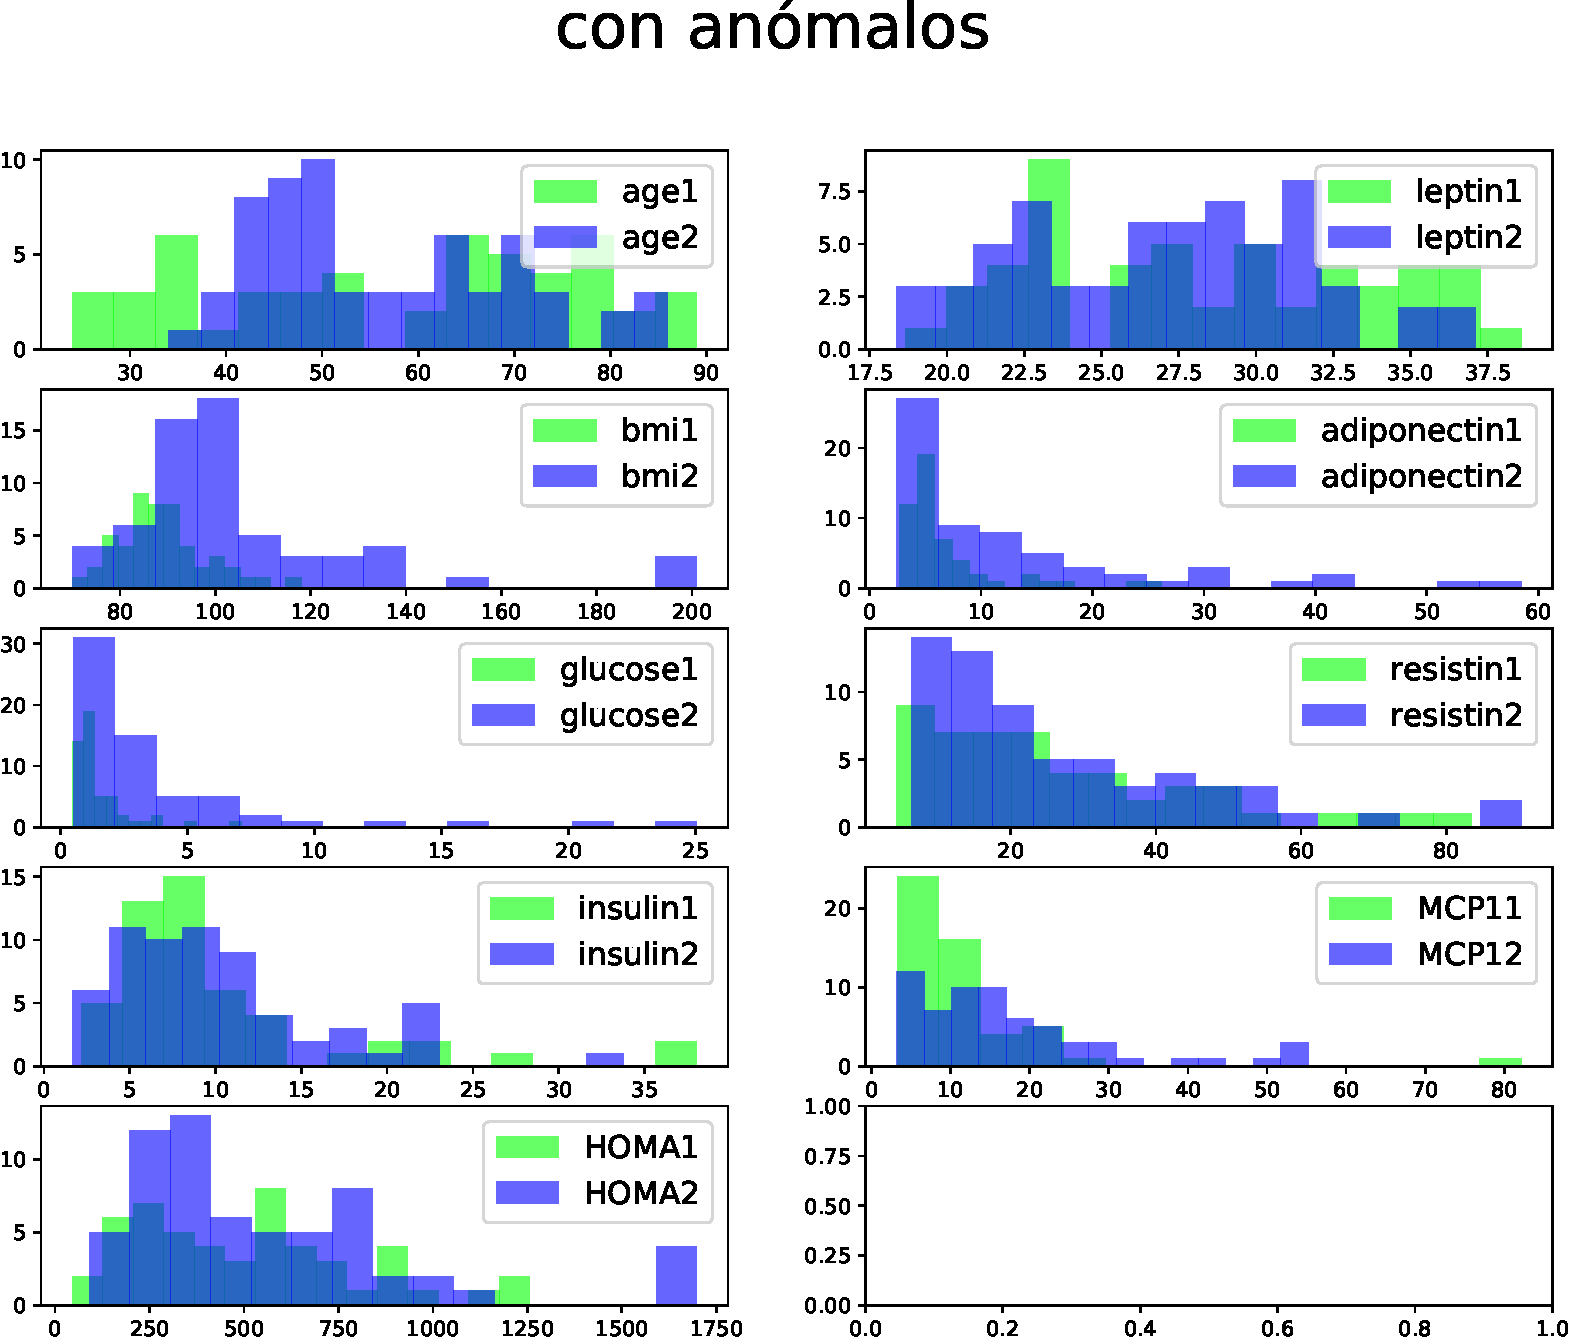
\includegraphics[width = 0.49\linewidth]{../python/images/hist.pdf}
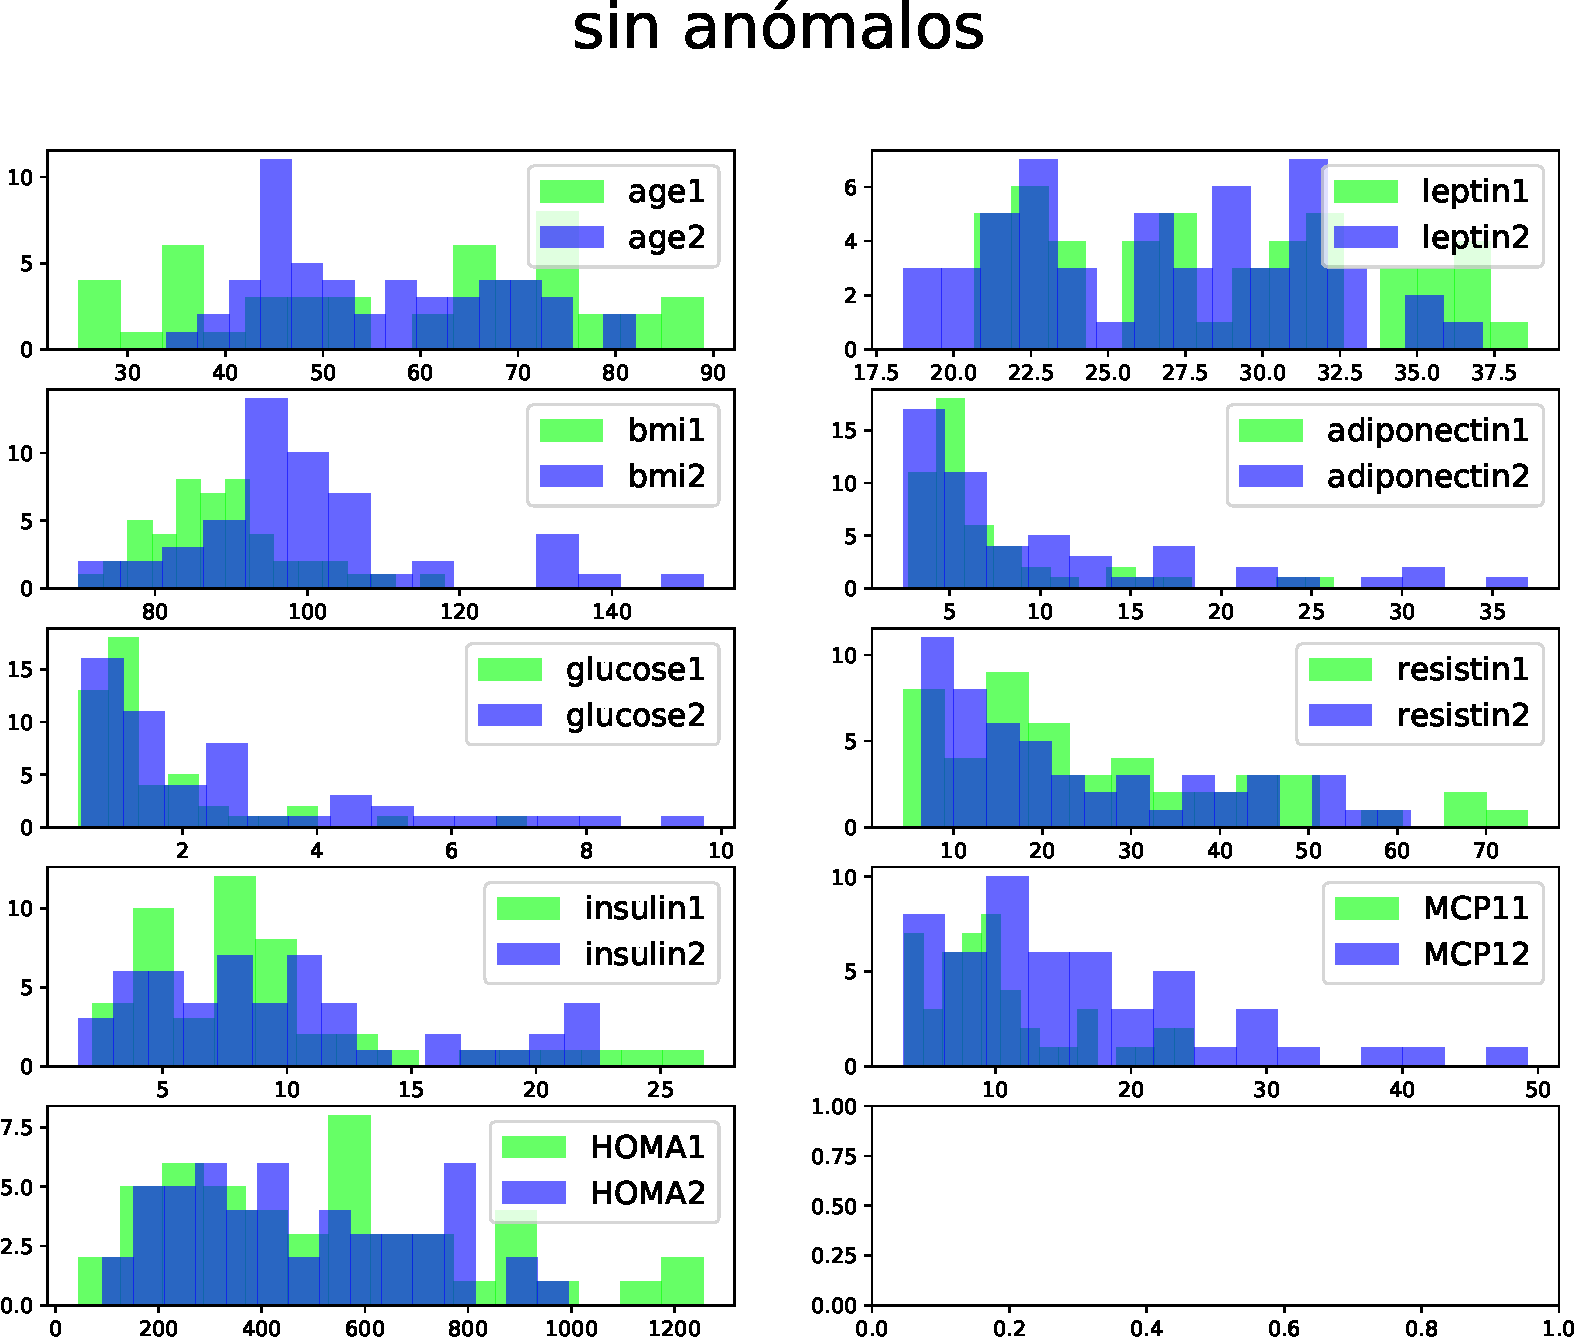
\includegraphics[width = 0.49\linewidth]{../python/images/hist1.pdf}
\figcaption{Histogramas Python para datos con y sin anomalias.}
\label{fig:histsP}
\end{figure}

\lstinputlisting[
	linerange = {9-30},
	caption = {[C\'odigo Python generador de los histogramas con datos an\'omalos.]
	\lstcaption{C\'odigo Python generador de los histogramas con datos an\'omalos.}},
	]{../python/src/histograms.py}

\newpage
\begin{figure}[h]
\centering
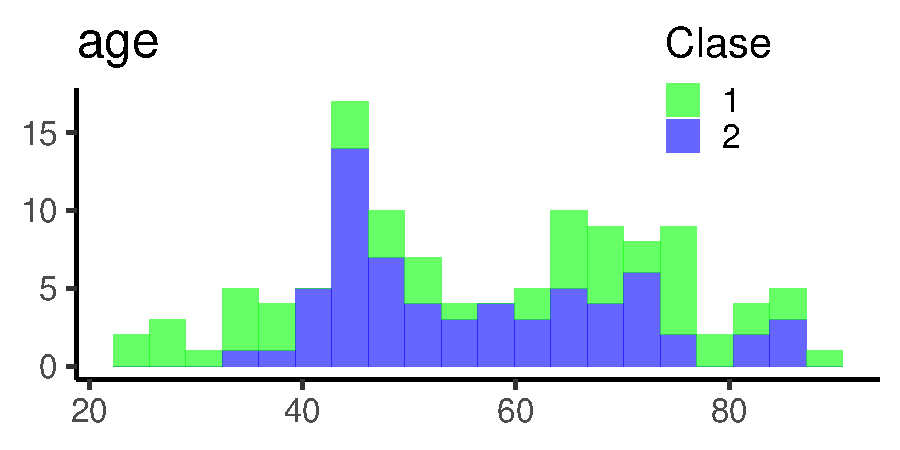
\includegraphics[width = 0.4\linewidth]{../R/images/hist1.pdf}
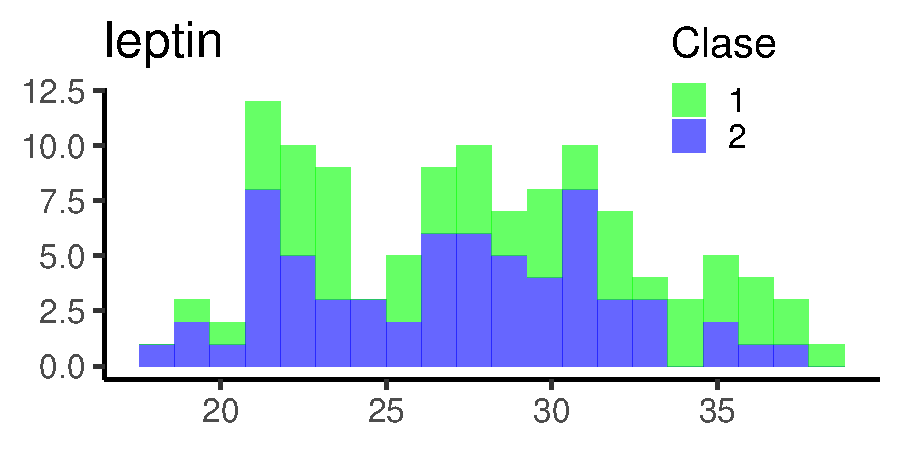
\includegraphics[width = 0.4\linewidth]{../R/images/hist2.pdf}
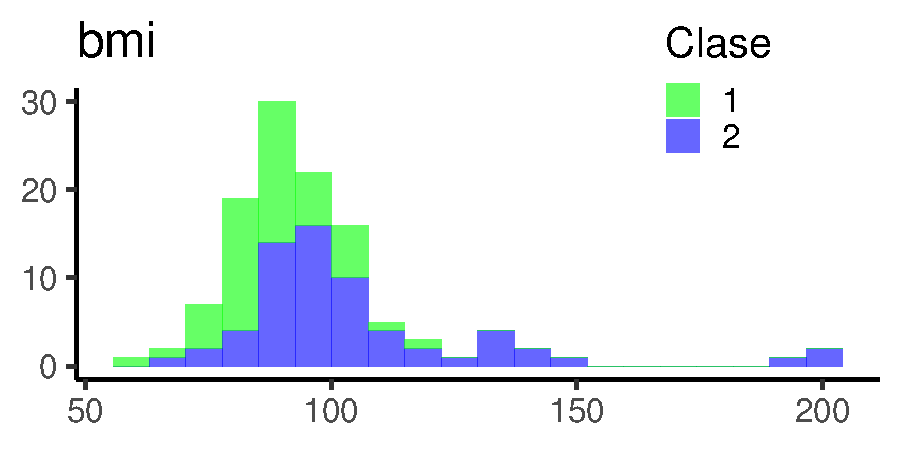
\includegraphics[width = 0.4\linewidth]{../R/images/hist3.pdf}
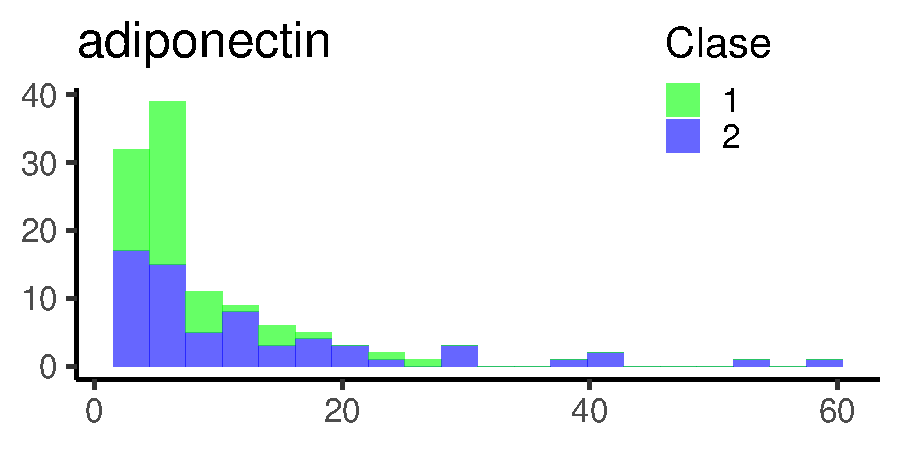
\includegraphics[width = 0.4\linewidth]{../R/images/hist4.pdf}
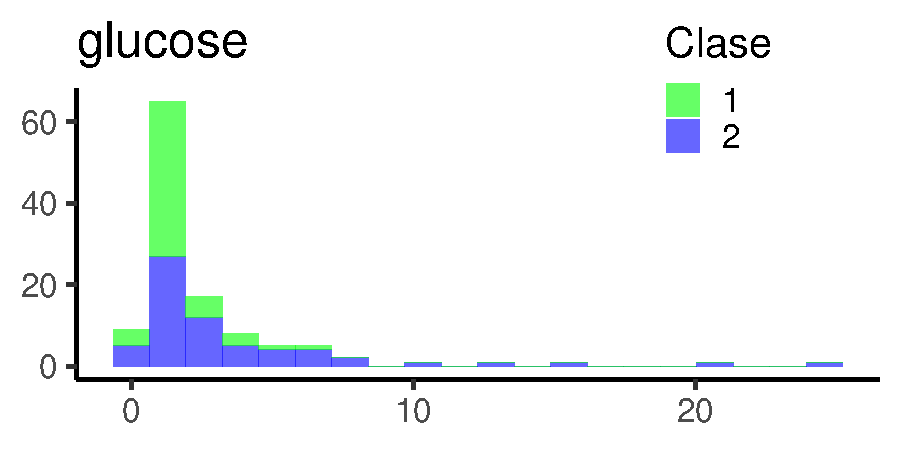
\includegraphics[width = 0.4\linewidth]{../R/images/hist5.pdf}
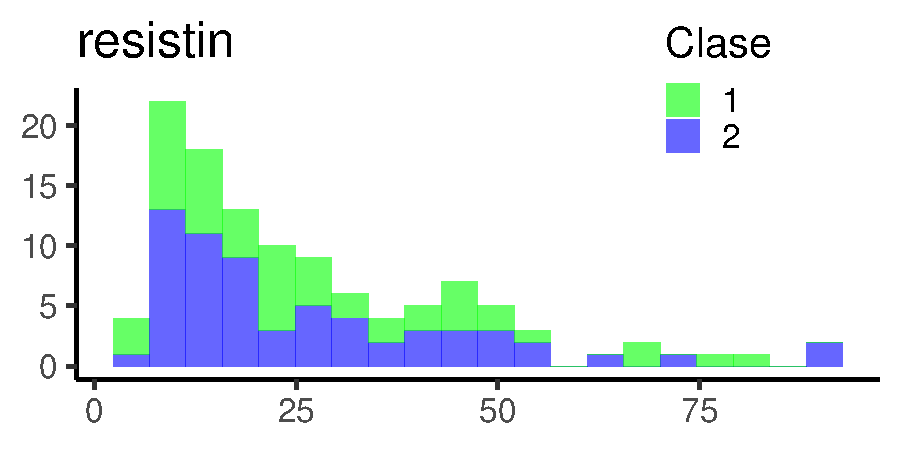
\includegraphics[width = 0.4\linewidth]{../R/images/hist6.pdf}
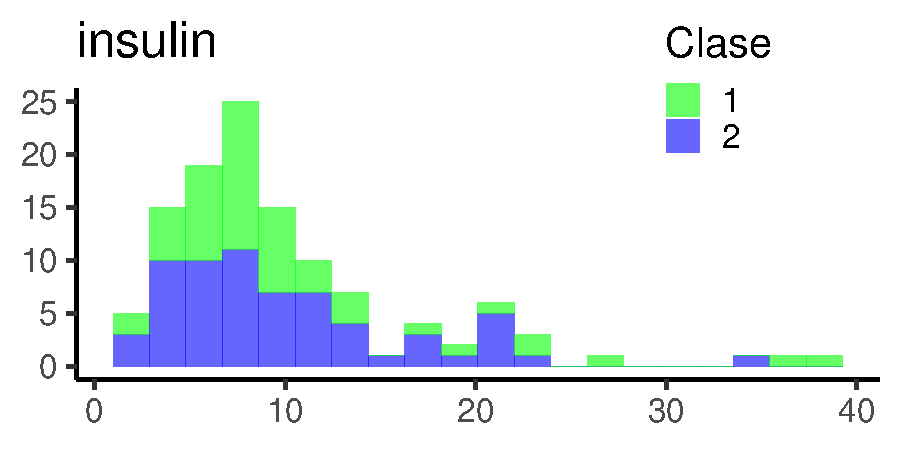
\includegraphics[width = 0.4\linewidth]{../R/images/hist7.pdf}
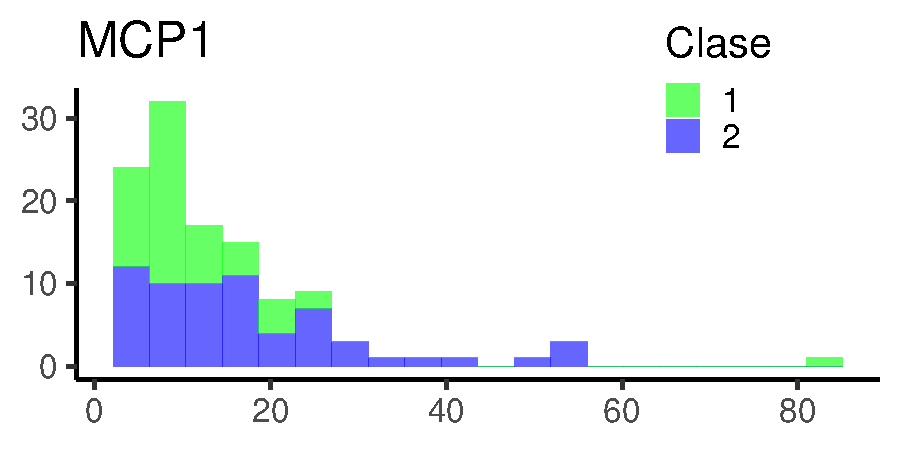
\includegraphics[width = 0.4\linewidth]{../R/images/hist8.pdf}
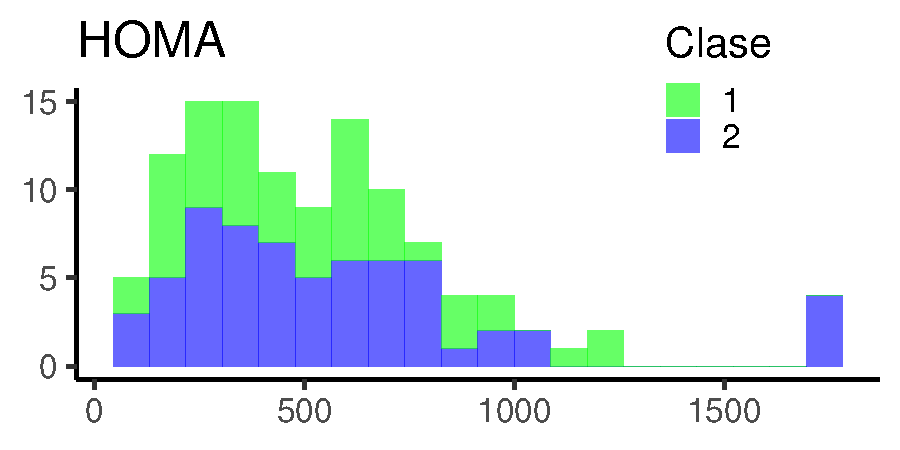
\includegraphics[width = 0.4\linewidth]{../R/images/hist9.pdf}
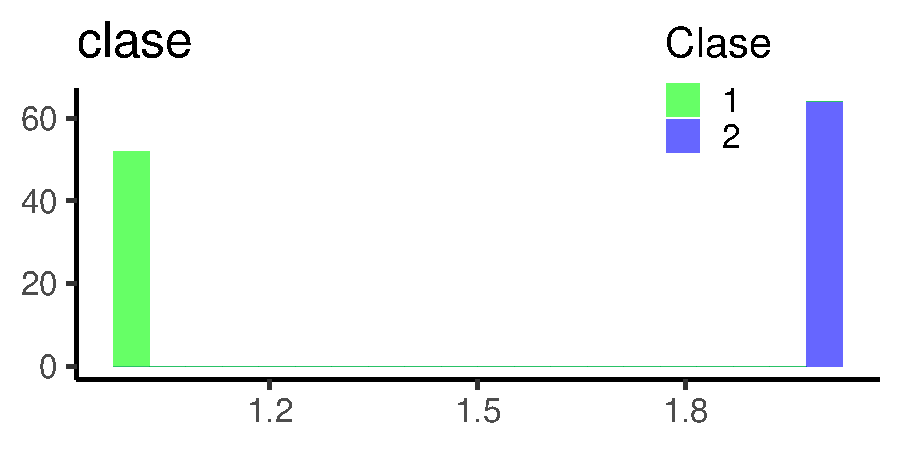
\includegraphics[width = 0.4\linewidth]{../R/images/hist10.pdf}
\figcaption{Histogramas R para datos con anomalias.}
\label{fig:histsR}
\end{figure}

\lstinputlisting[
	linerange = {8-18},
	caption = {[C\'odigo R generador de los histrogramas con datos an\'omalos.]
	\lstcaption{C\'odigo R generador de los histrogramas con datos an\'omalos.}},
	]{../R/src/histograms.r}

\newpage

\seccion{Kernel Density}

\begin{figure}[h]
\centering
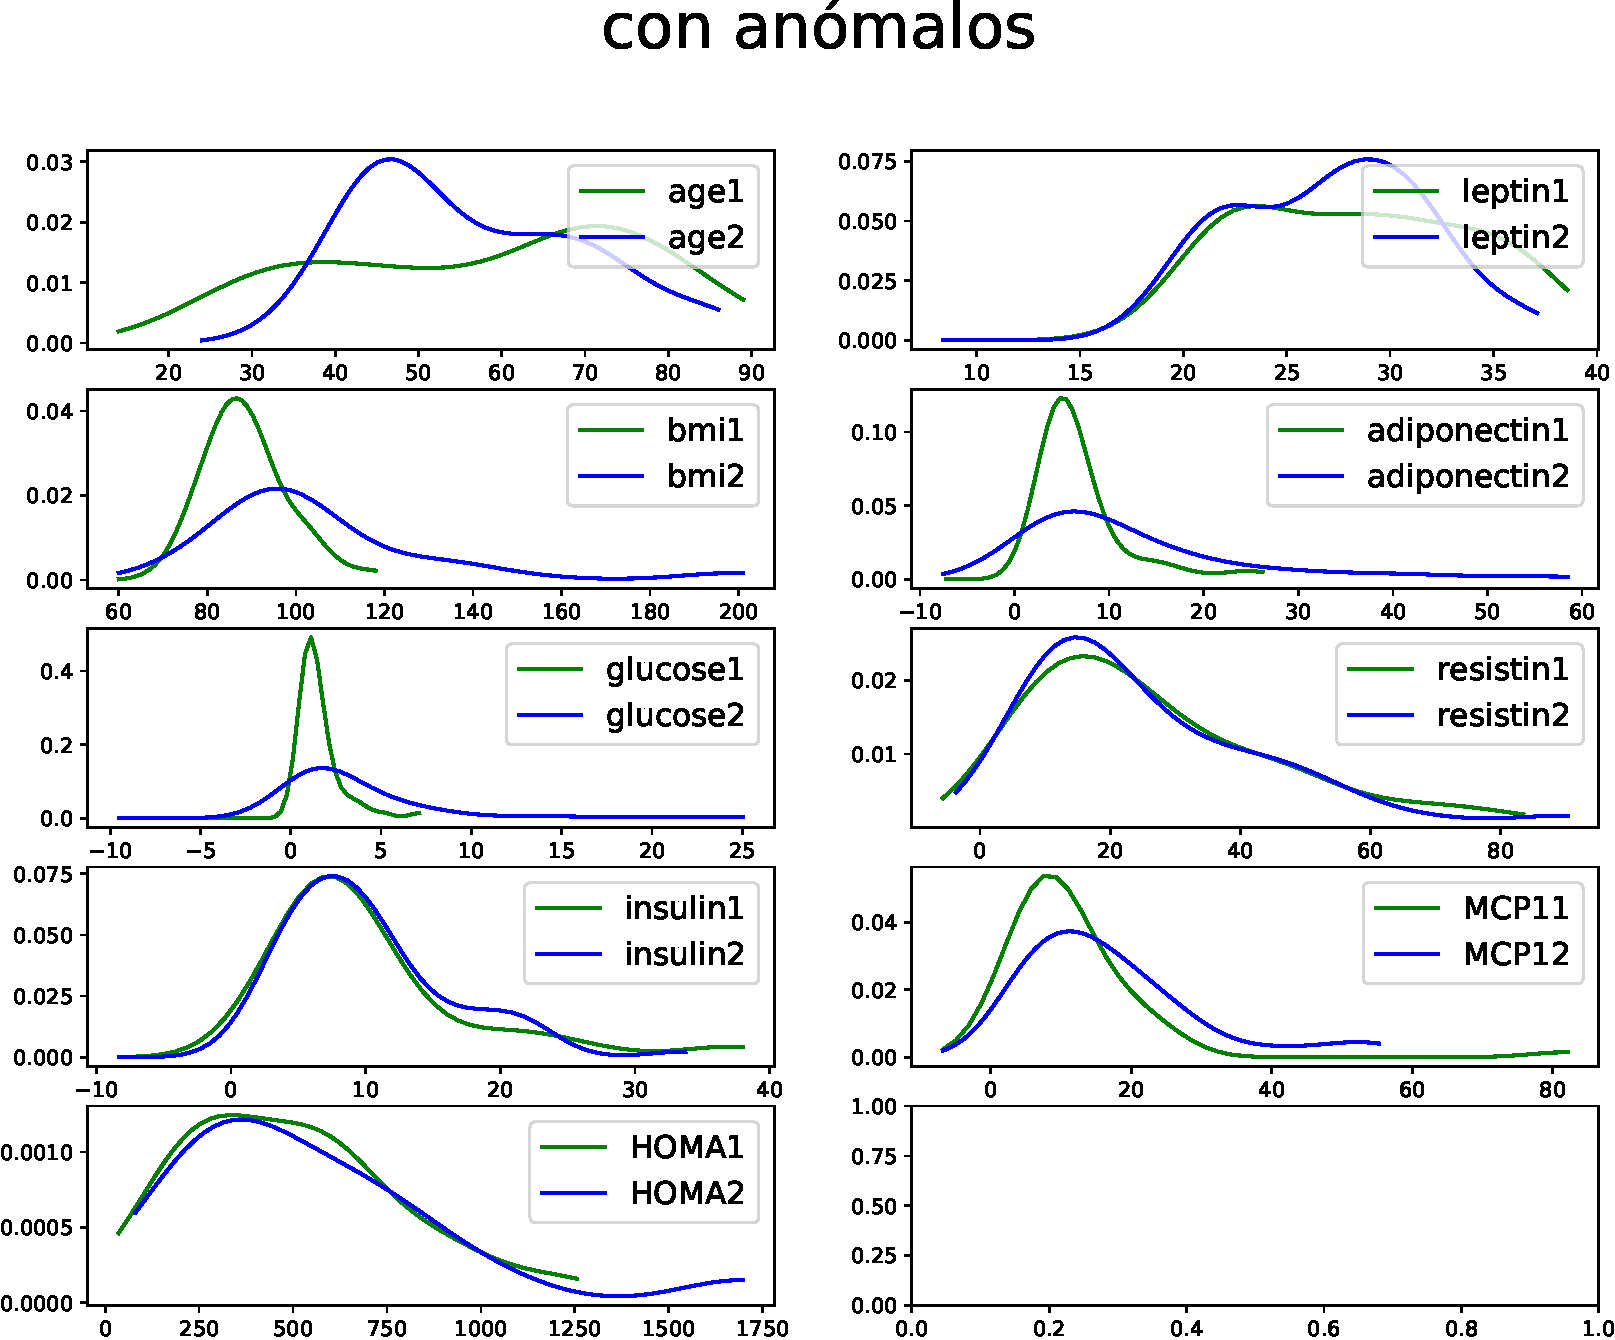
\includegraphics[width = 0.49\linewidth]{../python/images/kden.pdf}
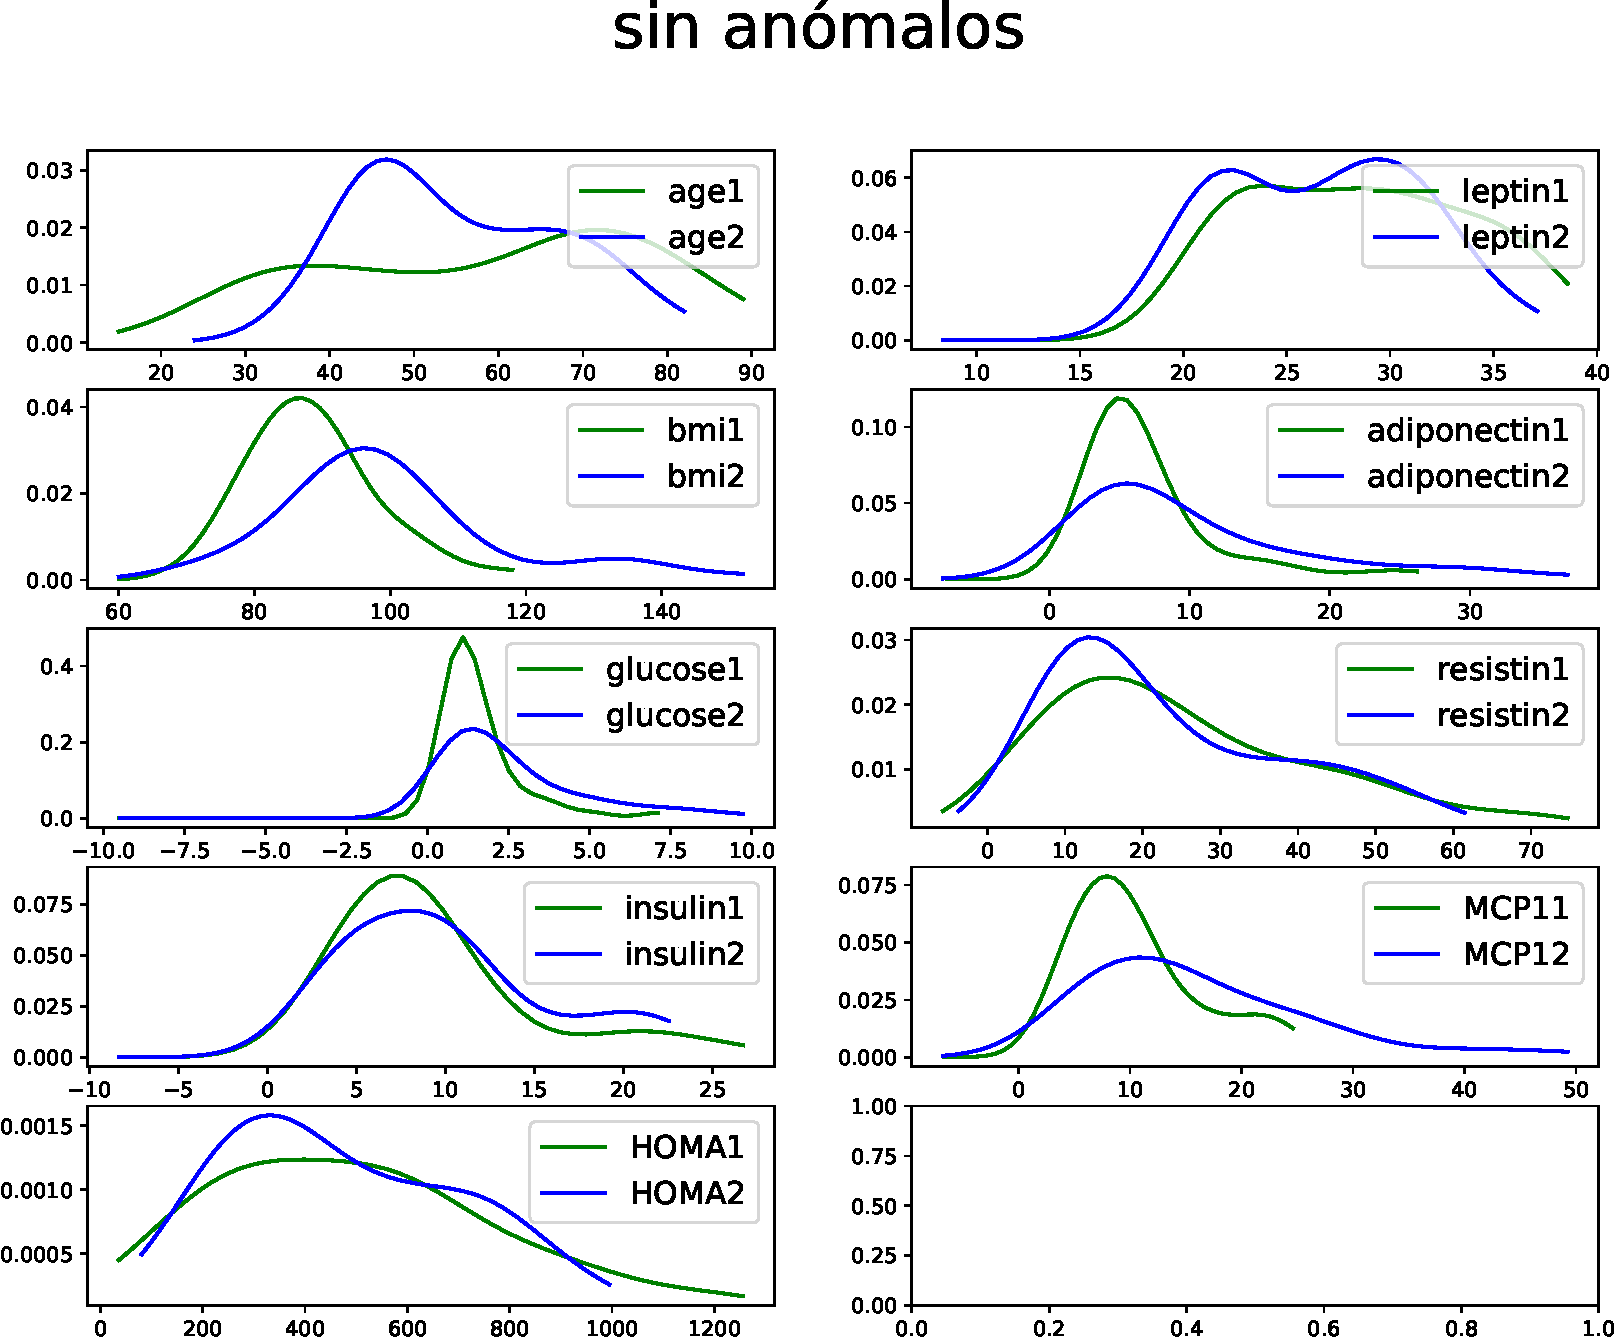
\includegraphics[width = 0.49\linewidth]{../python/images/kden1.pdf}
\figcaption{Kernel Density para datos con y sin anomalias.}
\label{fig:kdens}
\end{figure}

\lstinputlisting[
	linerange = {9-32},
	caption = {[C\'odigo Python generador de los kernel density plots con datos an\'omalos.]
	\lstcaption{C\'odigo Python generador de los kernel density plots con datos an\'omalos.}},
	]{../python/src/kerneldensity.py}
\newpage
\begin{figure}[h]
\centering
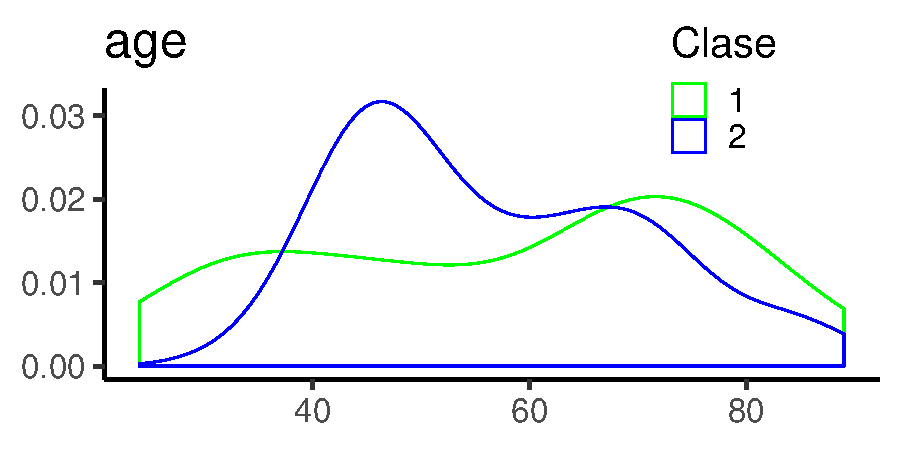
\includegraphics[width = 0.4\linewidth]{../R/images/dens1.pdf}
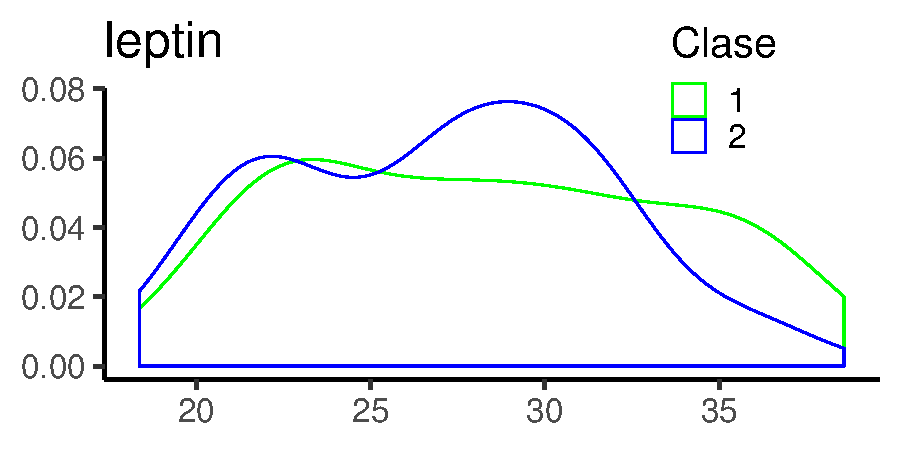
\includegraphics[width = 0.4\linewidth]{../R/images/dens2.pdf}
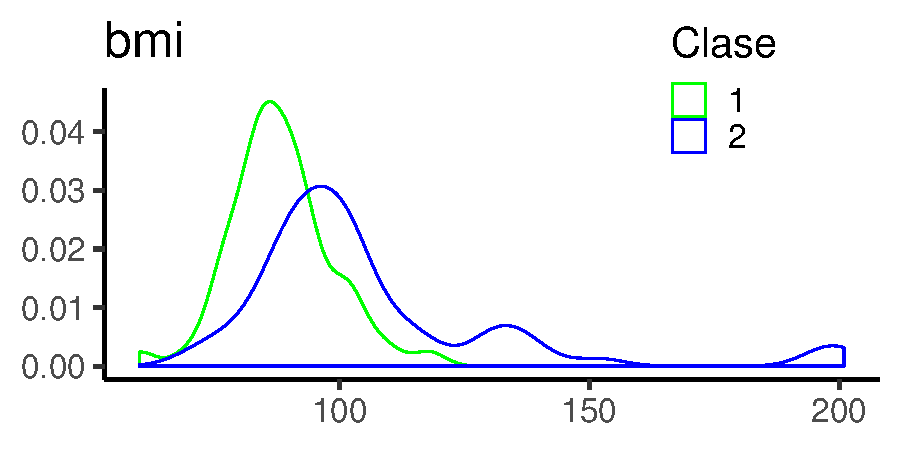
\includegraphics[width = 0.4\linewidth]{../R/images/dens3.pdf}
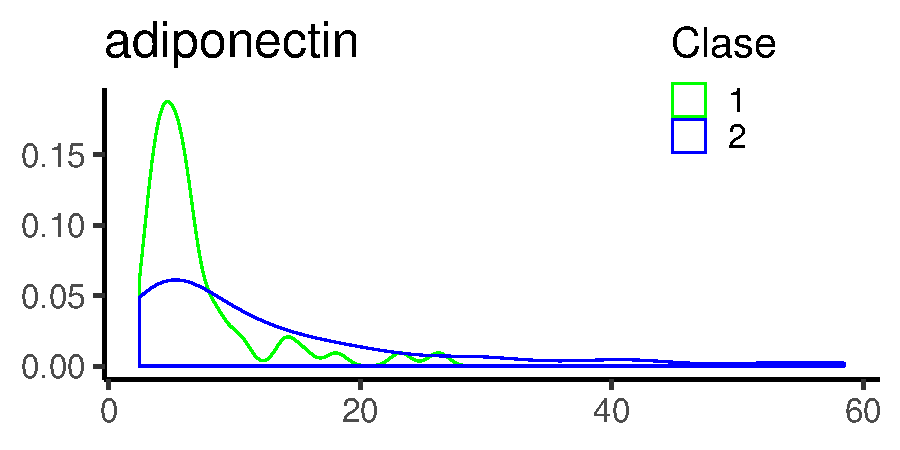
\includegraphics[width = 0.4\linewidth]{../R/images/dens4.pdf}
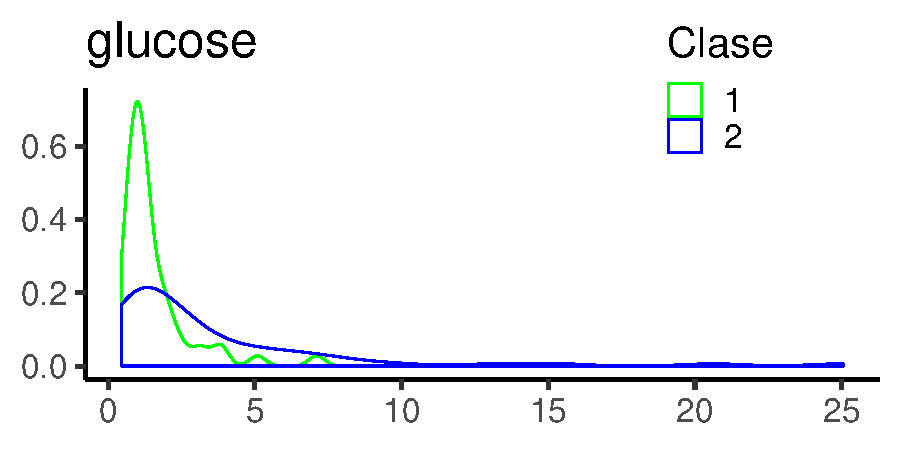
\includegraphics[width = 0.4\linewidth]{../R/images/dens5.pdf}
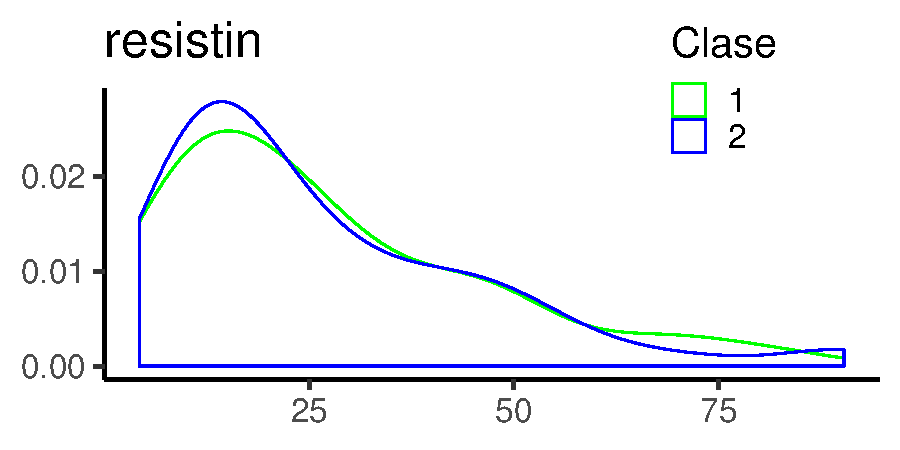
\includegraphics[width = 0.4\linewidth]{../R/images/dens6.pdf}
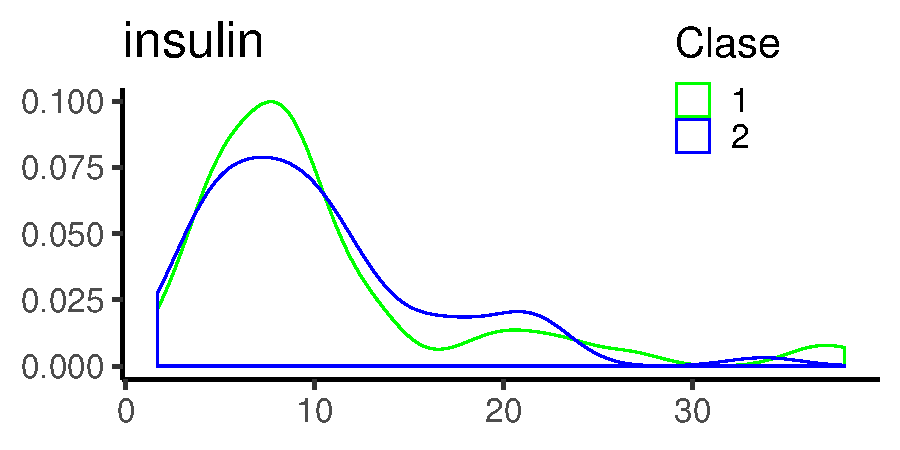
\includegraphics[width = 0.4\linewidth]{../R/images/dens7.pdf}
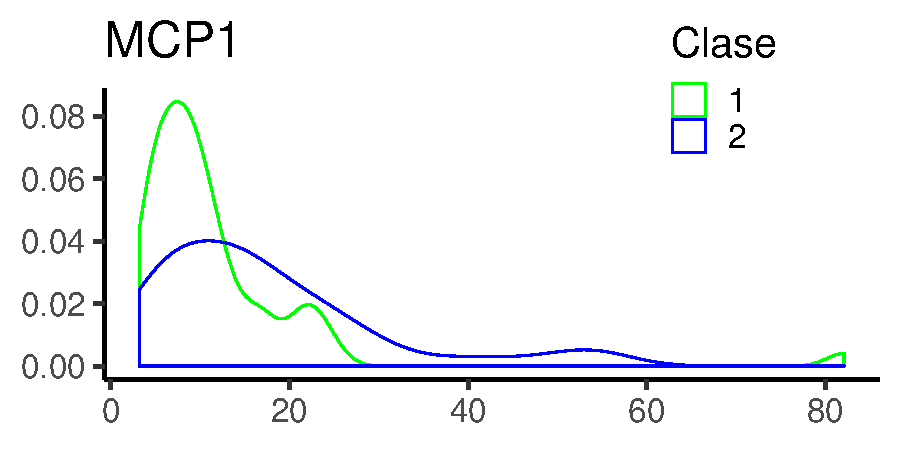
\includegraphics[width = 0.4\linewidth]{../R/images/dens8.pdf}
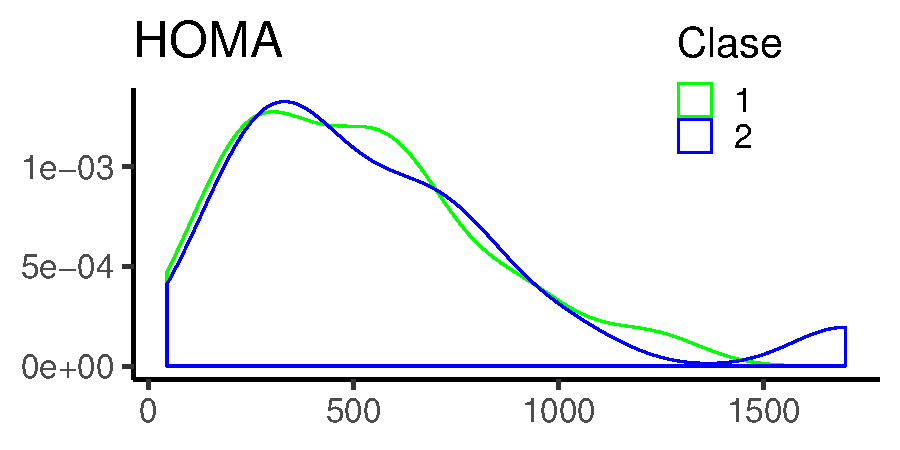
\includegraphics[width = 0.4\linewidth]{../R/images/dens9.pdf}
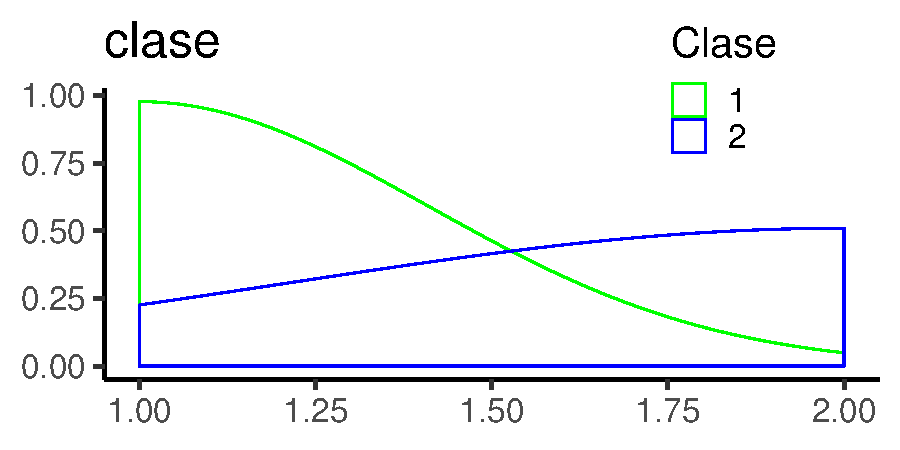
\includegraphics[width = 0.4\linewidth]{../R/images/dens10.pdf}
\figcaption{Gr\'aficos de densidad R.}
\label{fig:densR}
\end{figure}

\lstinputlisting[
	linerange = {8-18},
	caption = {[C\'odigo R generador de los density plots.]
	\lstcaption{C\'odigo R generador de los density plots.}},
	]{../R/src/kerneldensity.r}
\newpage

\seccion{Boxplot}

\begin{figure}[h]
\centering
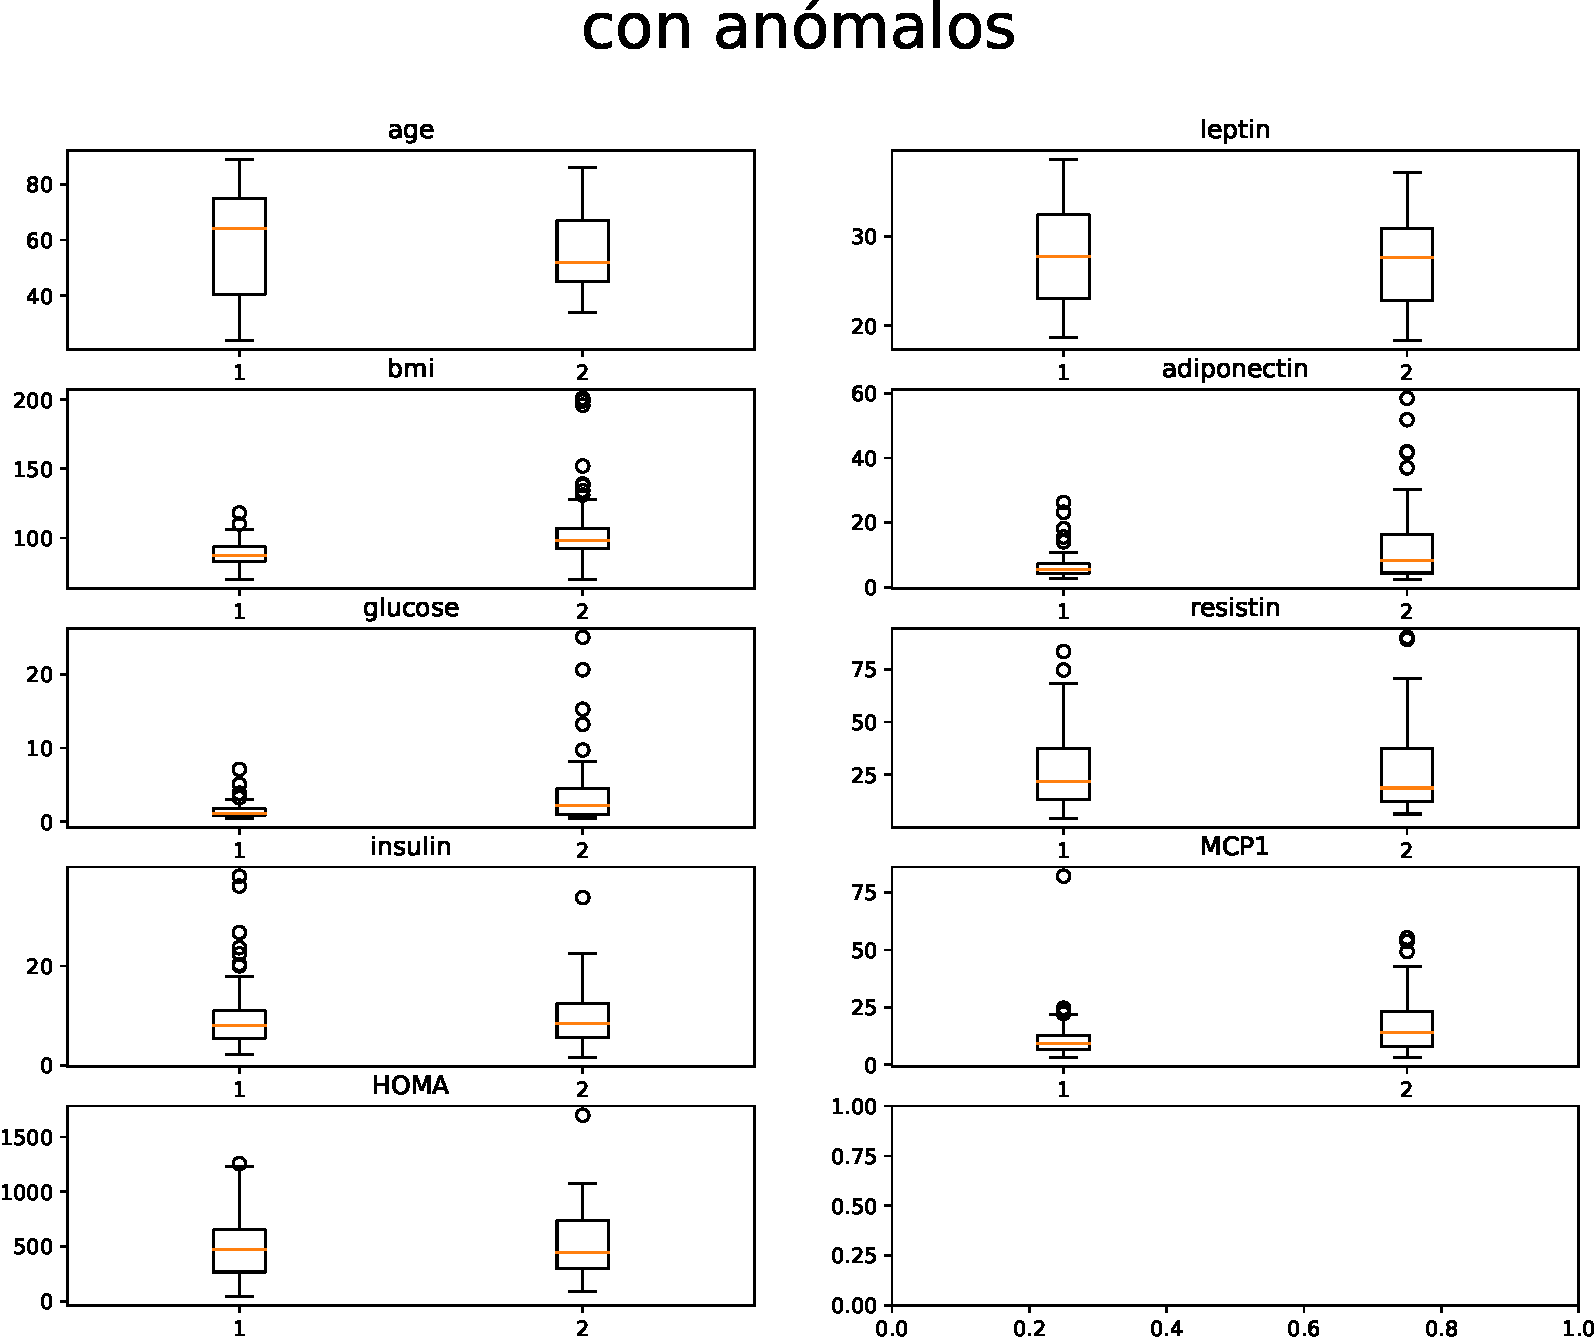
\includegraphics[width = 0.49\linewidth]{../python/images/boxp.pdf}
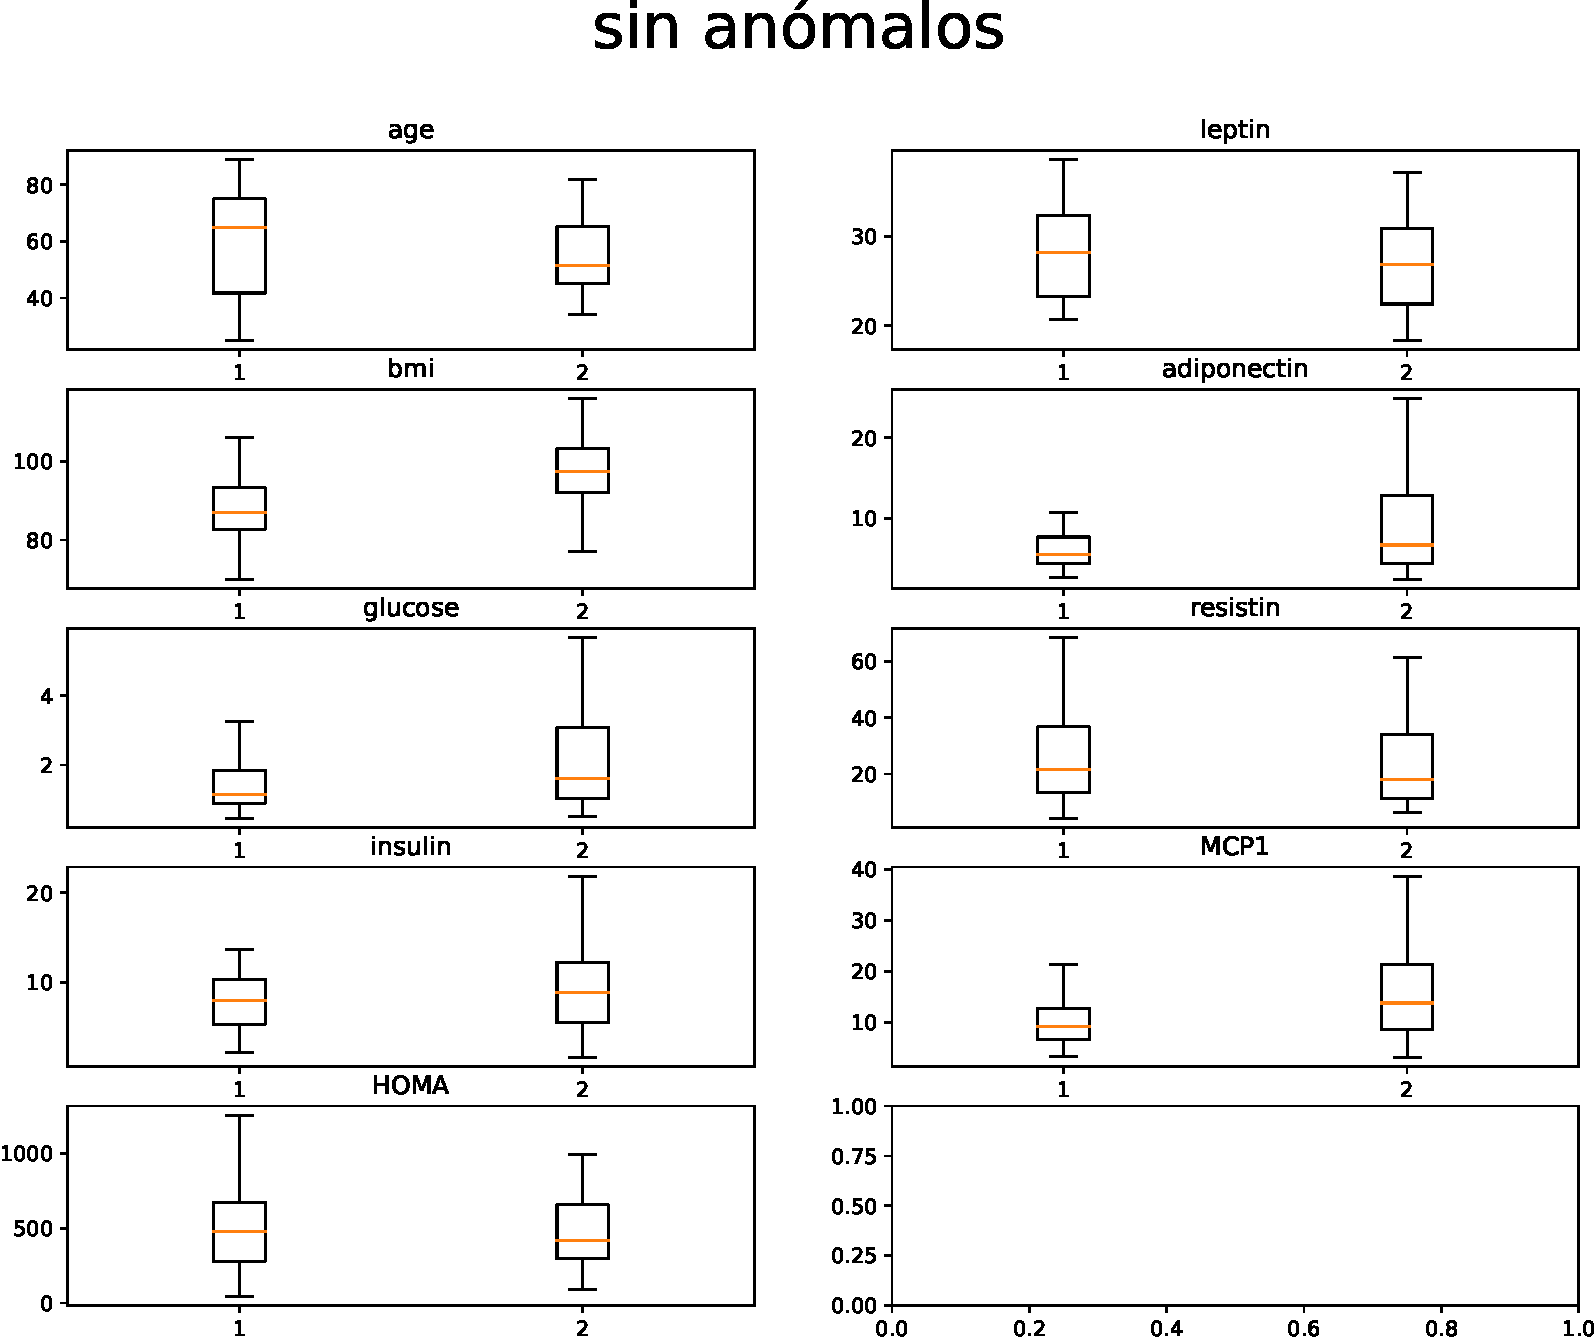
\includegraphics[width = 0.49\linewidth]{../python/images/boxp1.pdf}
\figcaption{Boxplots Python para datos con y sin anomalias.}
\label{fig:boxP}
\end{figure}

\lstinputlisting[
	linerange = {9-24},
	caption = {[C\'odigo Python generador de los boxplots con datos an\'omalos.]
	\lstcaption{C\'odigo Python generador de los boxplots con datos an\'omalos.}},
	]{../python/src/boxplot.py}

\newpage

\begin{figure}[h]
\centering
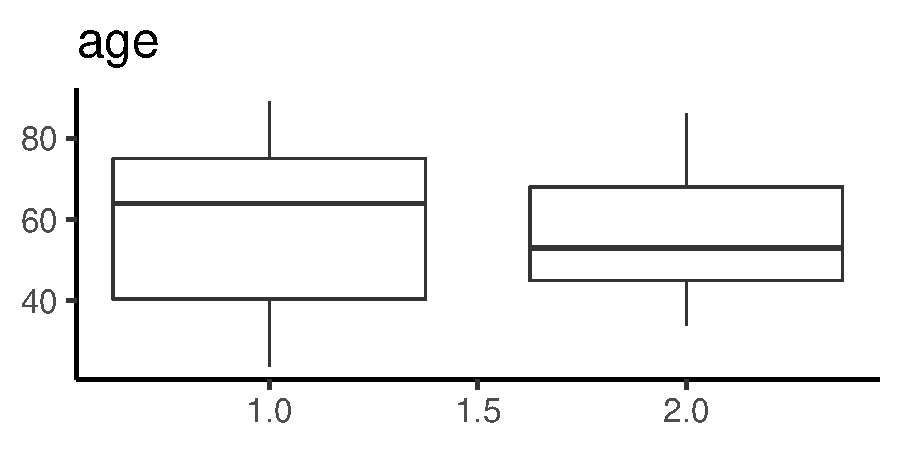
\includegraphics[width = 0.4\linewidth]{../R/images/box1.pdf}
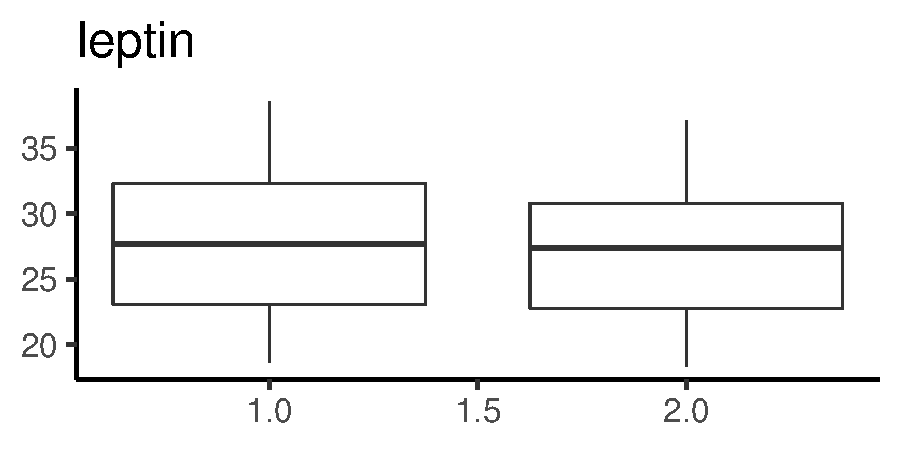
\includegraphics[width = 0.4\linewidth]{../R/images/box2.pdf}
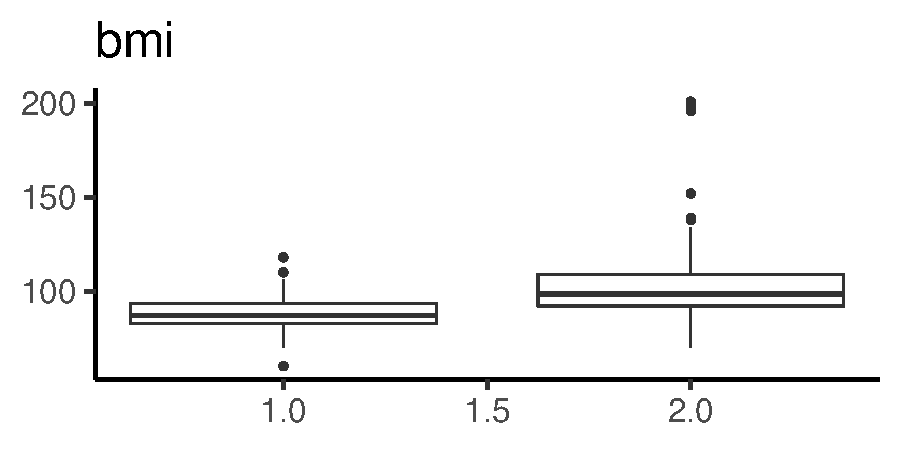
\includegraphics[width = 0.4\linewidth]{../R/images/box3.pdf}
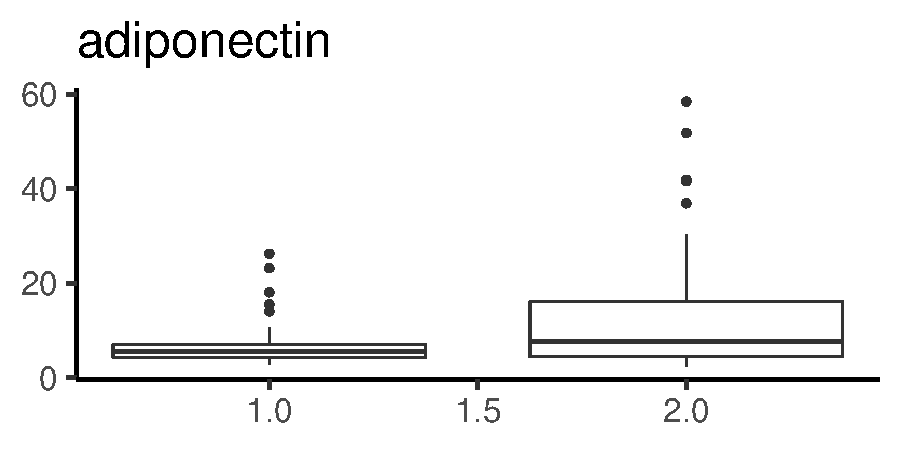
\includegraphics[width = 0.4\linewidth]{../R/images/box4.pdf}
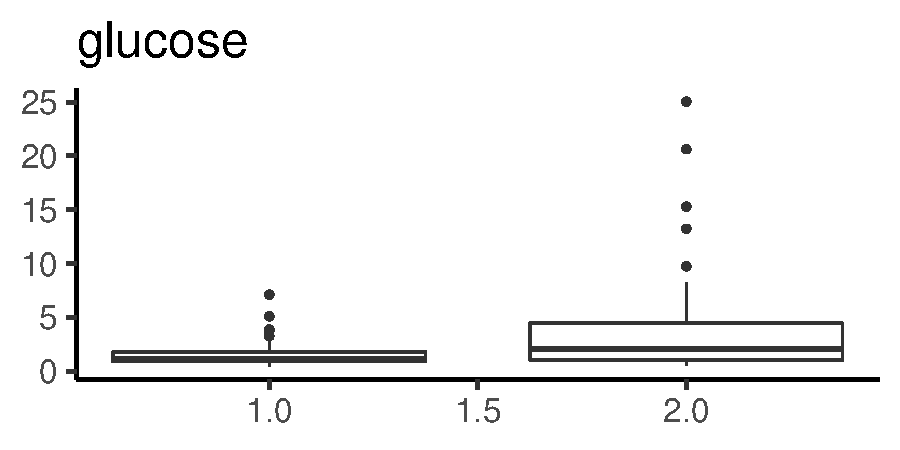
\includegraphics[width = 0.4\linewidth]{../R/images/box5.pdf}
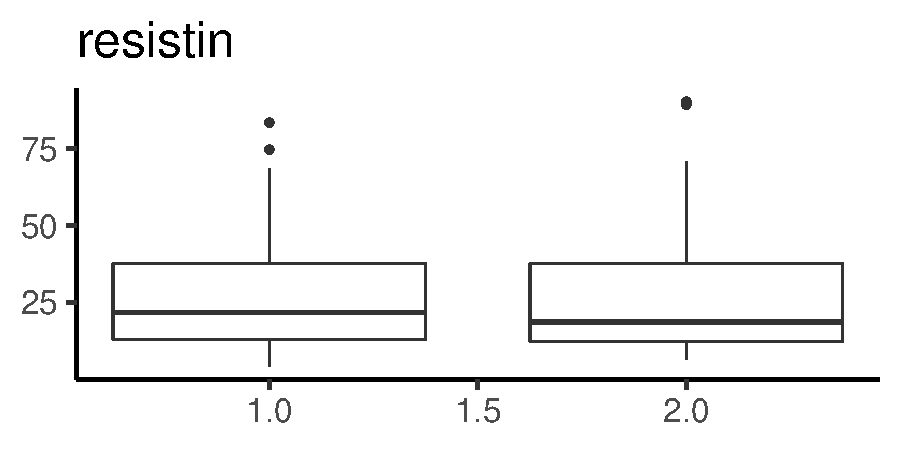
\includegraphics[width = 0.4\linewidth]{../R/images/box6.pdf}
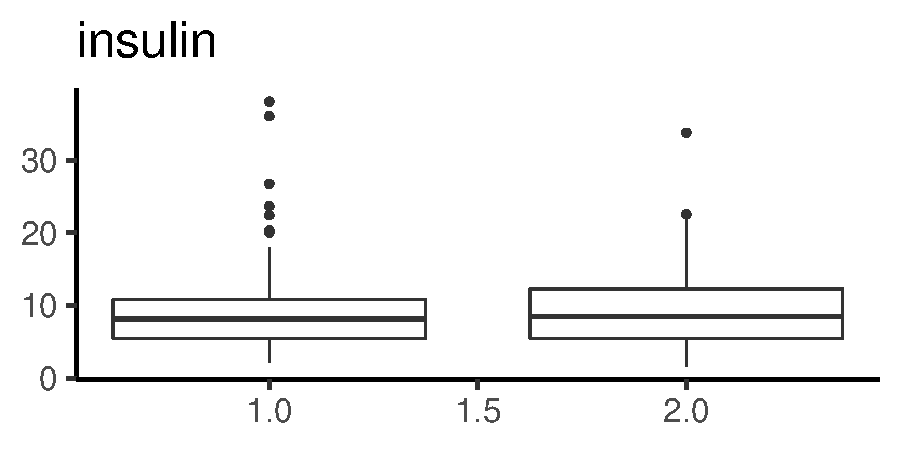
\includegraphics[width = 0.4\linewidth]{../R/images/box7.pdf}
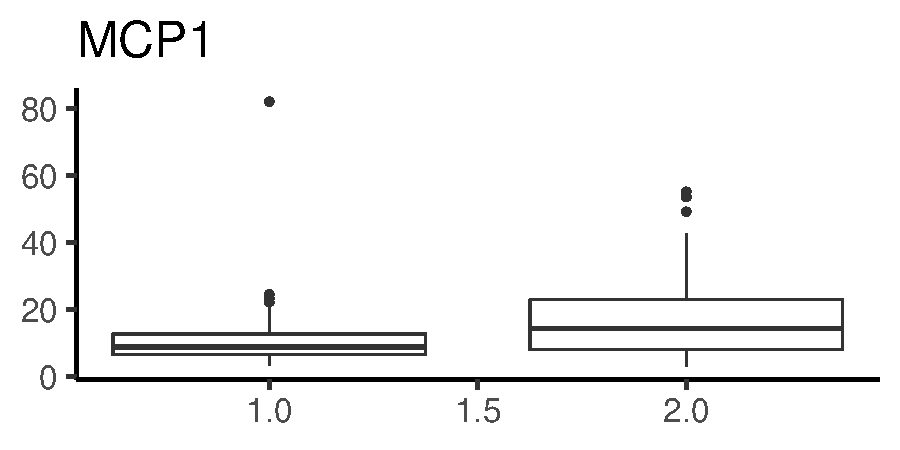
\includegraphics[width = 0.4\linewidth]{../R/images/box8.pdf}
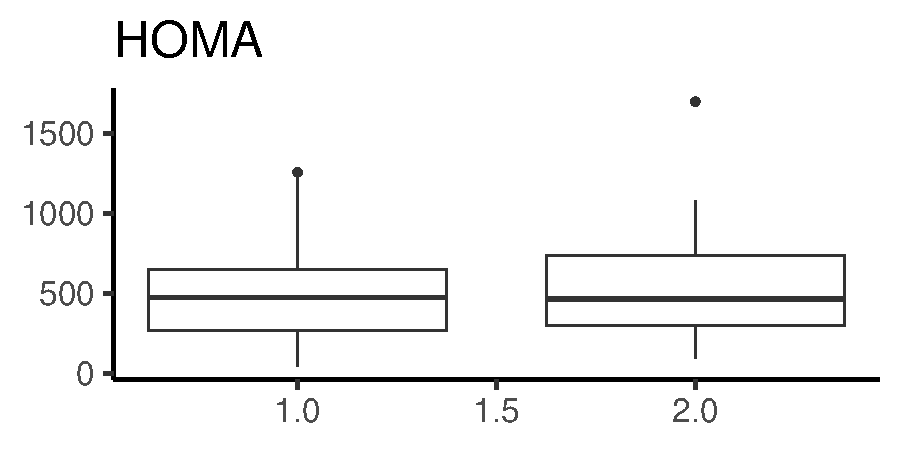
\includegraphics[width = 0.4\linewidth]{../R/images/box9.pdf}
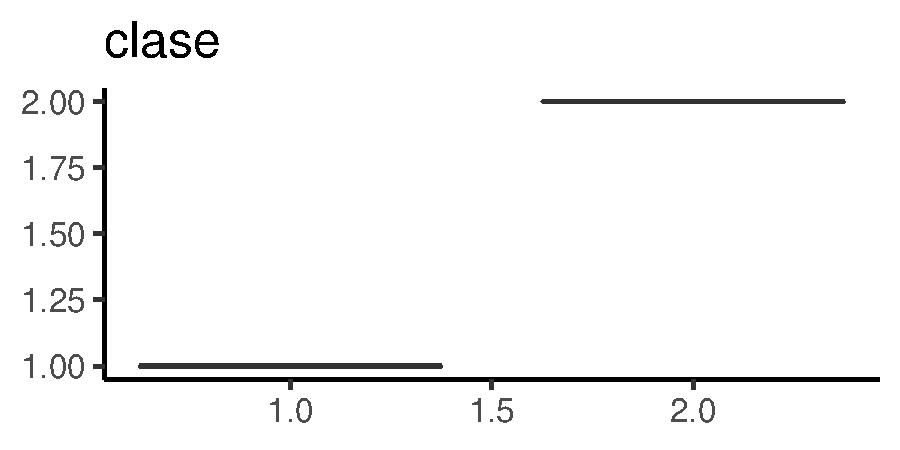
\includegraphics[width = 0.4\linewidth]{../R/images/box10.pdf}
\figcaption{Boxplots R para datos con anomalias.}
\label{fig:boxR}
\end{figure}

\lstinputlisting[
	linerange = {8-18},
	caption = {[C\'odigo R generador de los boxplots con datos an\'omalos.]
	\lstcaption{C\'odigo R generador de los boxplots con datos an\'omalos.}},
	]{../R/src/boxplot.r}

\newpage
\seccion{QQplot}

\begin{figure}[h]
\centering
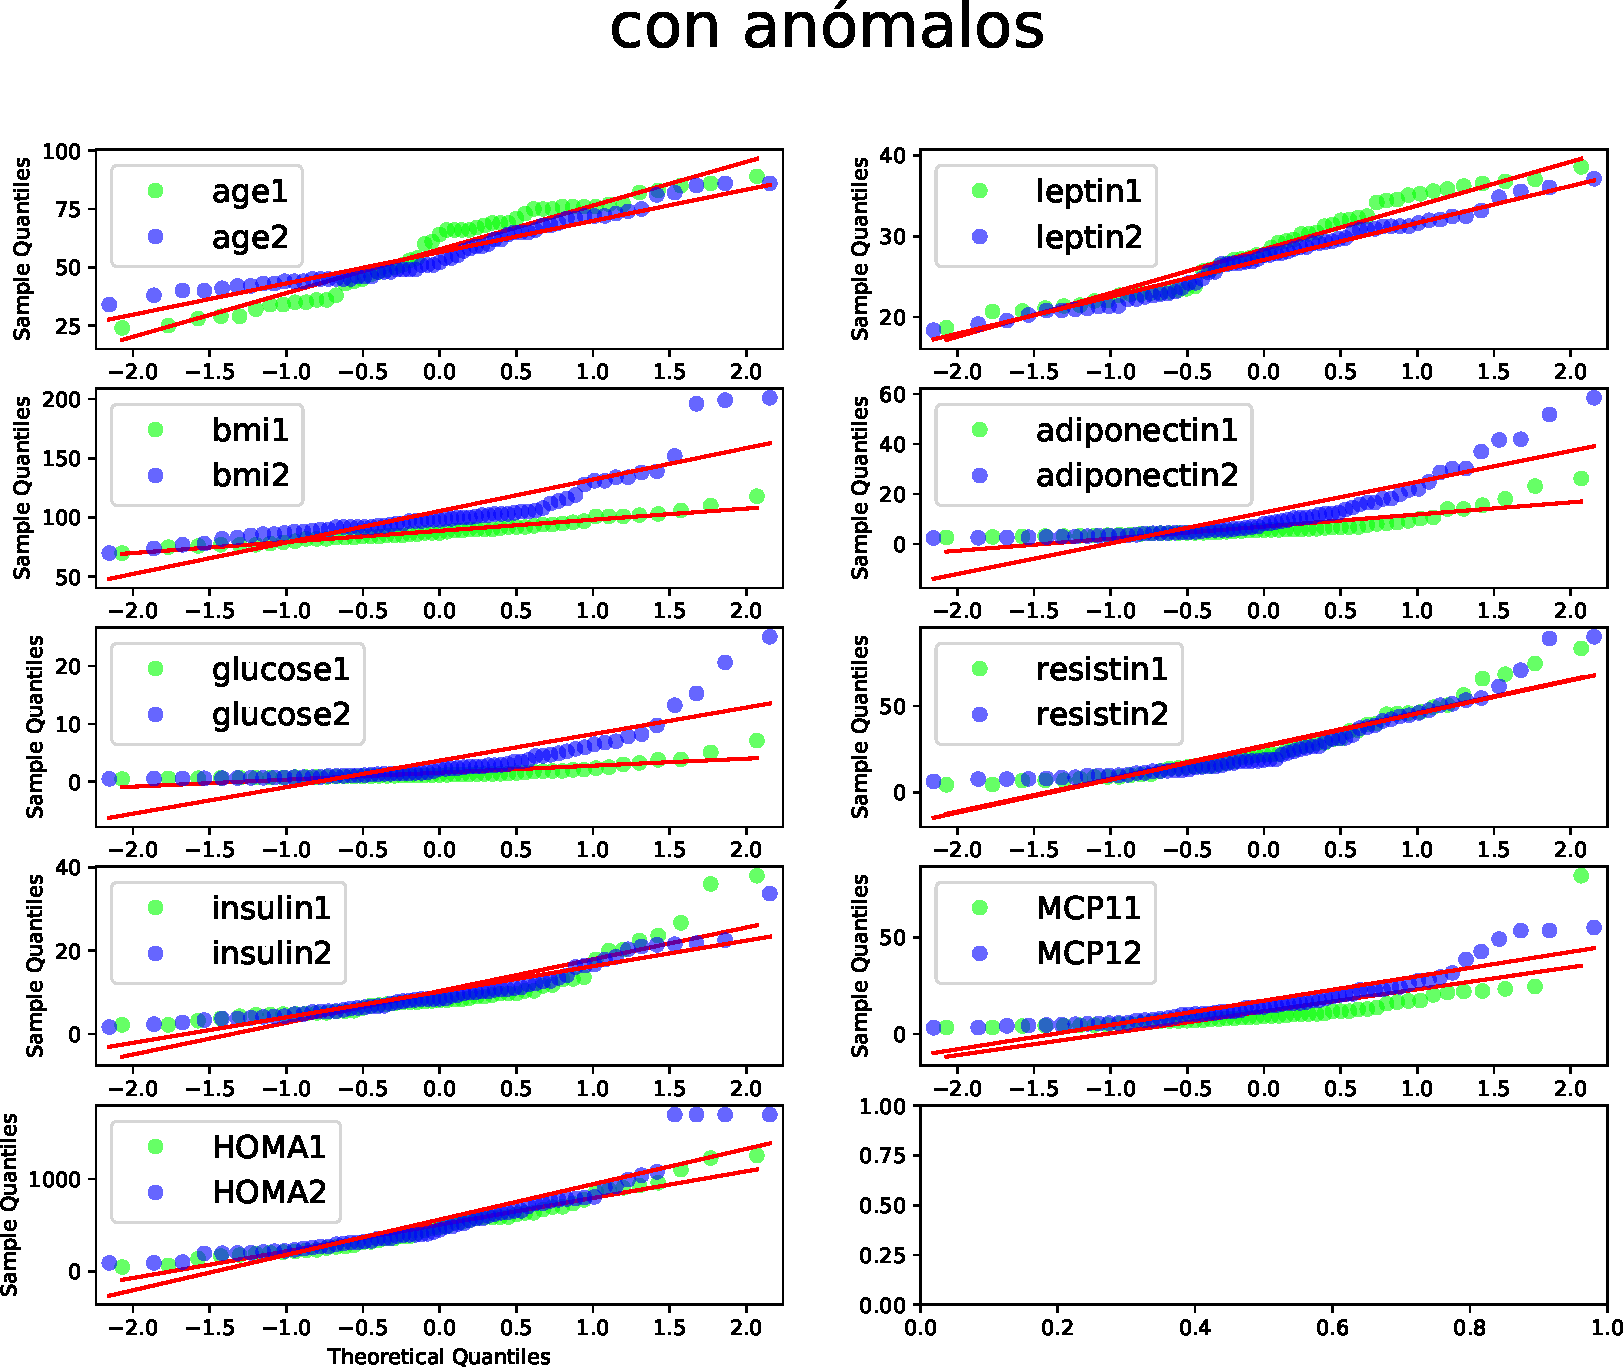
\includegraphics[width = 0.49\linewidth]{../python/images/qqp.pdf}
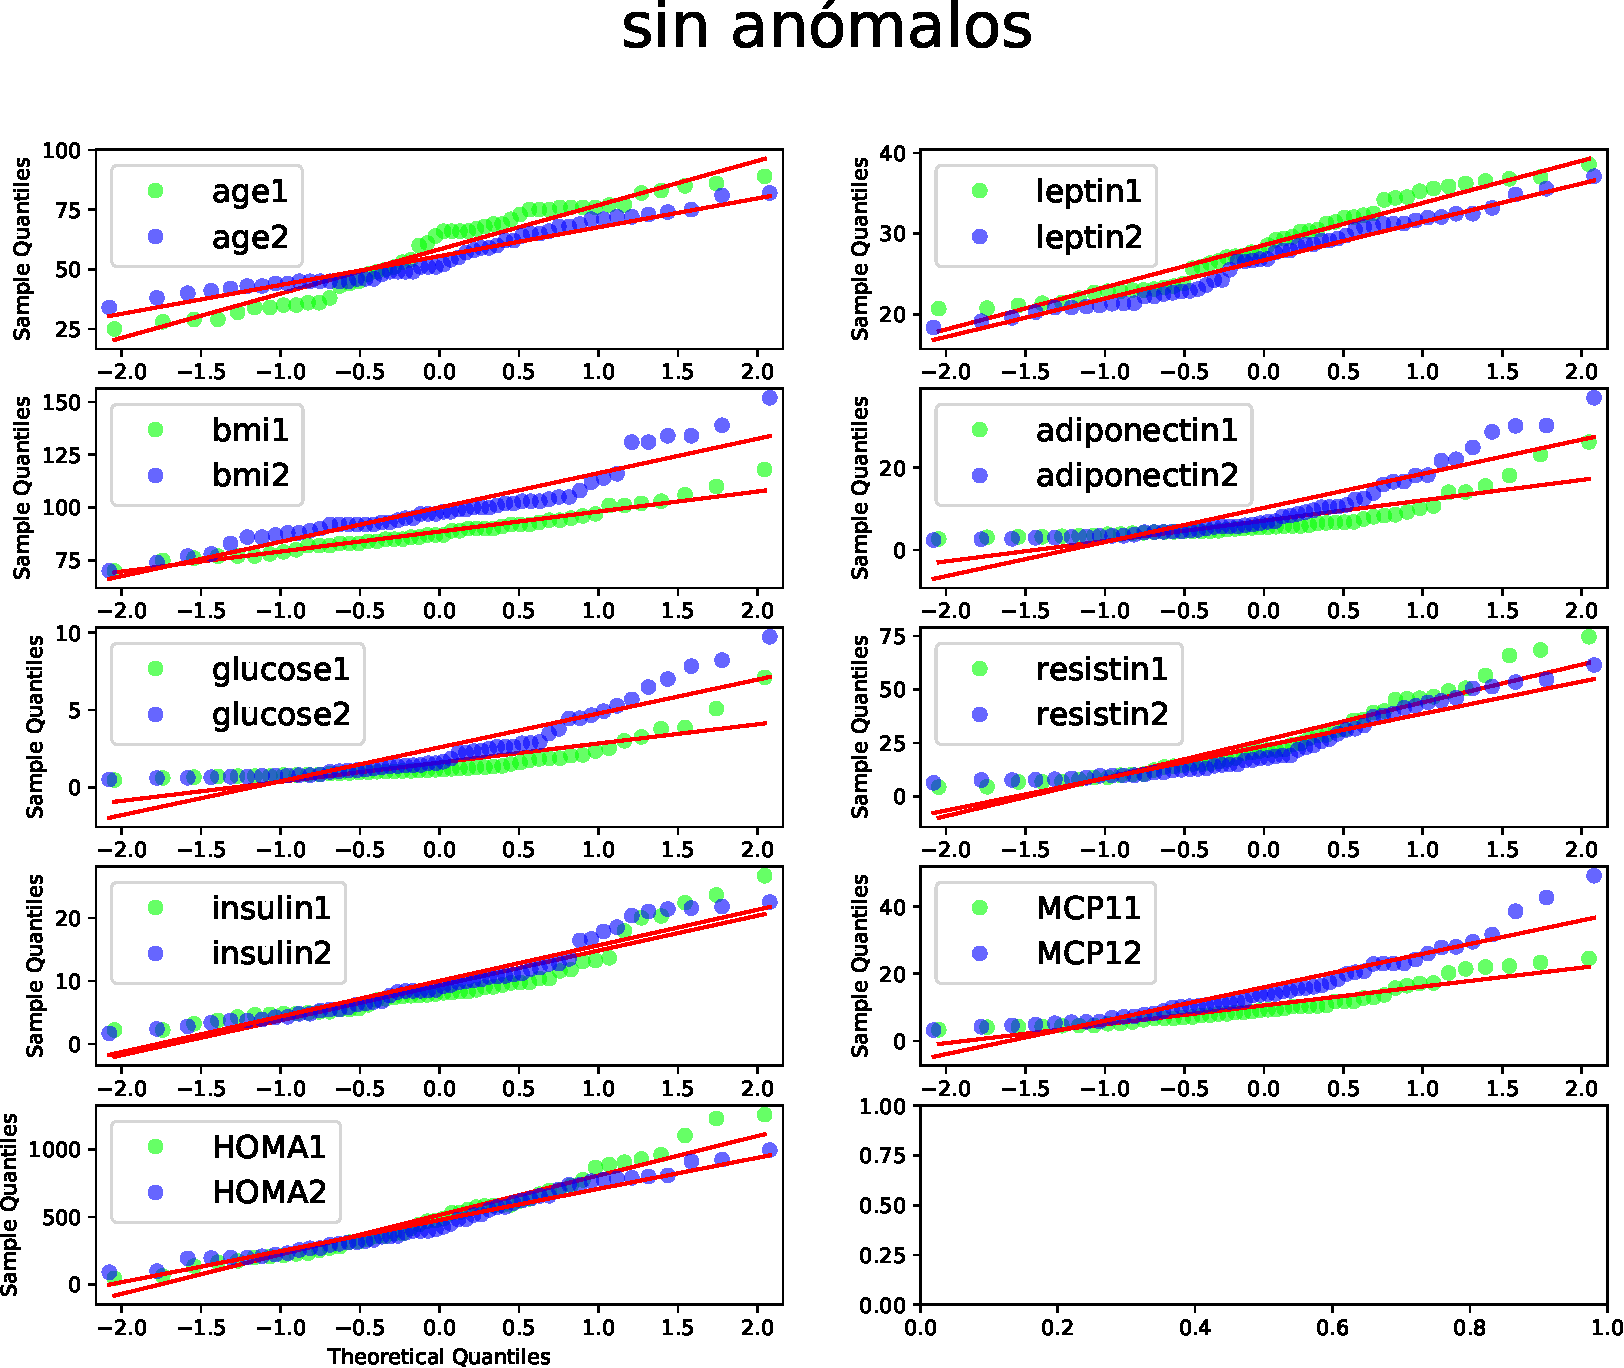
\includegraphics[width = 0.49\linewidth]{../python/images/qqp1.pdf}
\figcaption{QQplots Python para datos con y sin anomalias.}
\label{fig:qqps}
\end{figure}

\lstinputlisting[
	linerange = {9-28},
	caption = {[C\'odigo Python generador de los QQplots con datos an\'omalos.]
	\lstcaption{C\'odigo Python generador de los QQplots con datos an\'omalos.}},
	]{../python/src/qqplot.py}

\newpage
\begin{figure}[h]
\centering
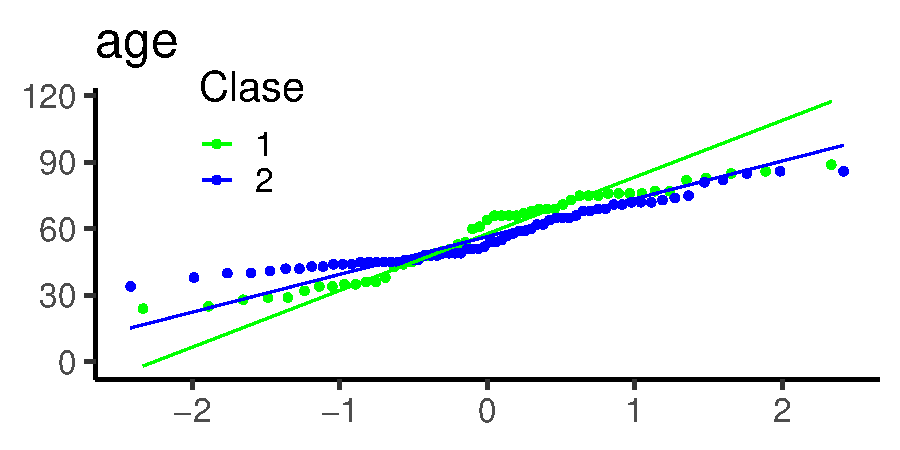
\includegraphics[width = 0.4\linewidth]{../R/images/qq1.pdf}
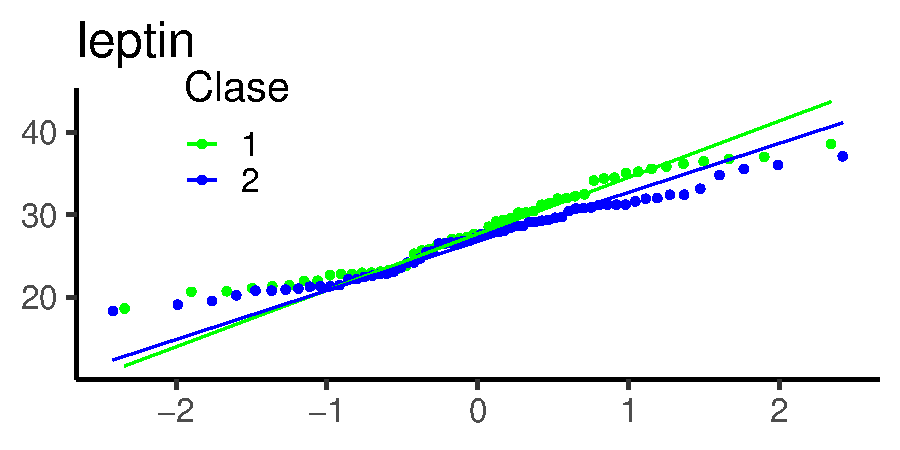
\includegraphics[width = 0.4\linewidth]{../R/images/qq2.pdf}
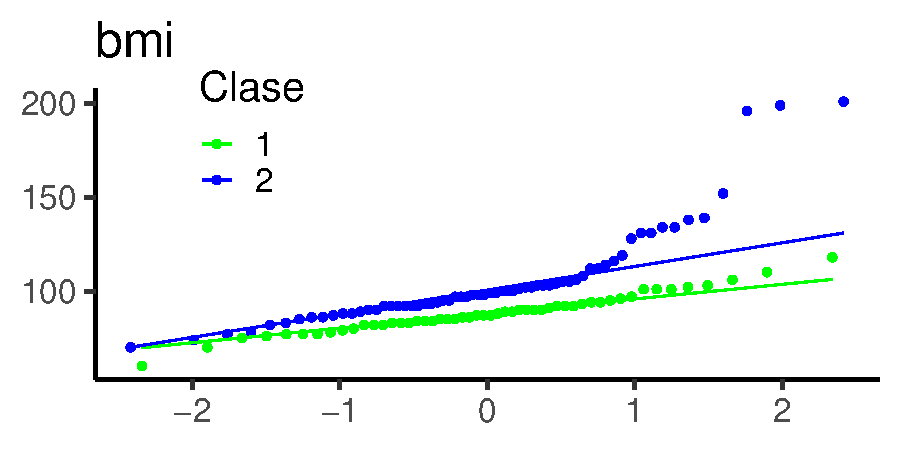
\includegraphics[width = 0.4\linewidth]{../R/images/qq3.pdf}
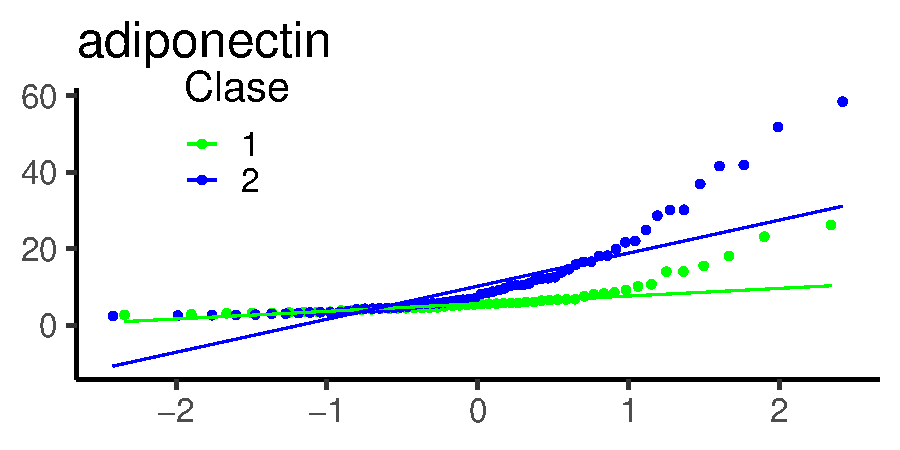
\includegraphics[width = 0.4\linewidth]{../R/images/qq4.pdf}
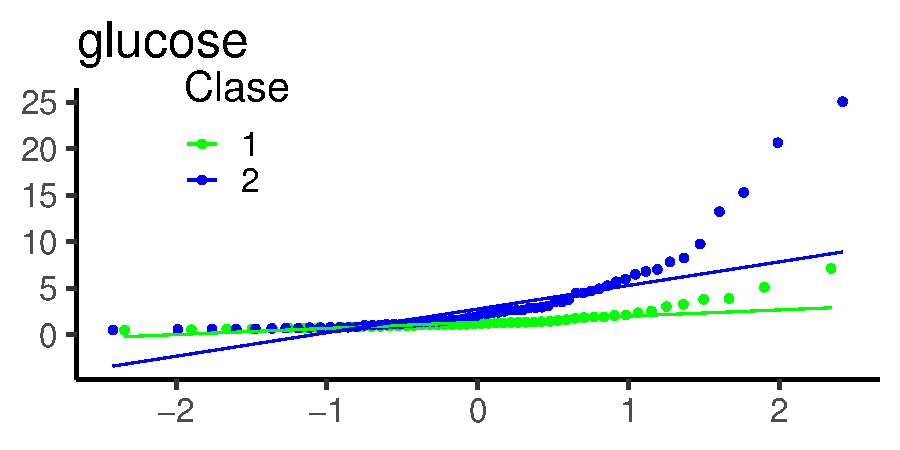
\includegraphics[width = 0.4\linewidth]{../R/images/qq5.pdf}
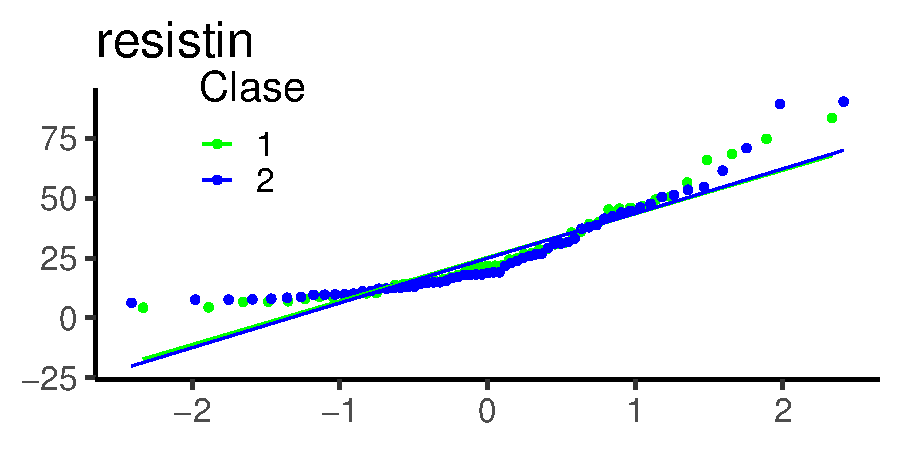
\includegraphics[width = 0.4\linewidth]{../R/images/qq6.pdf}
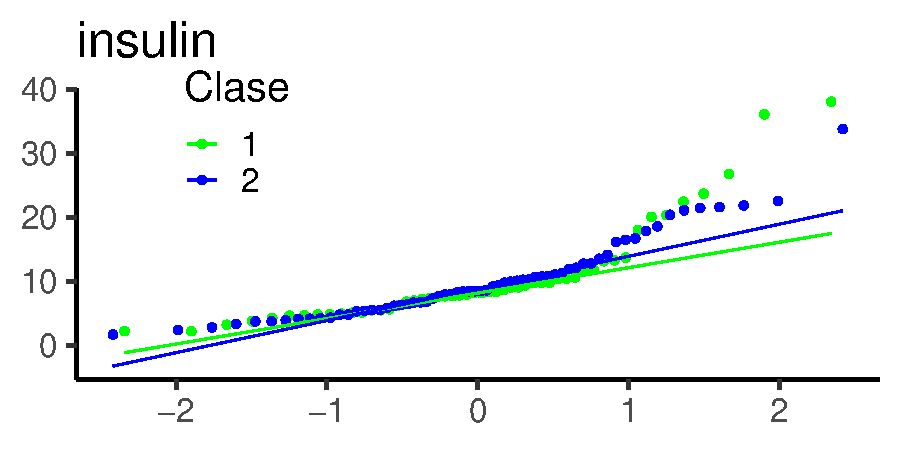
\includegraphics[width = 0.4\linewidth]{../R/images/qq7.pdf}
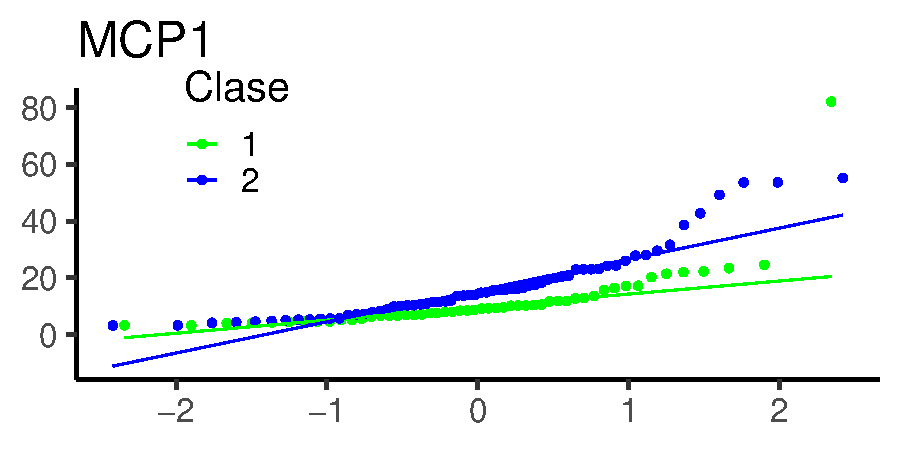
\includegraphics[width = 0.4\linewidth]{../R/images/qq8.pdf}
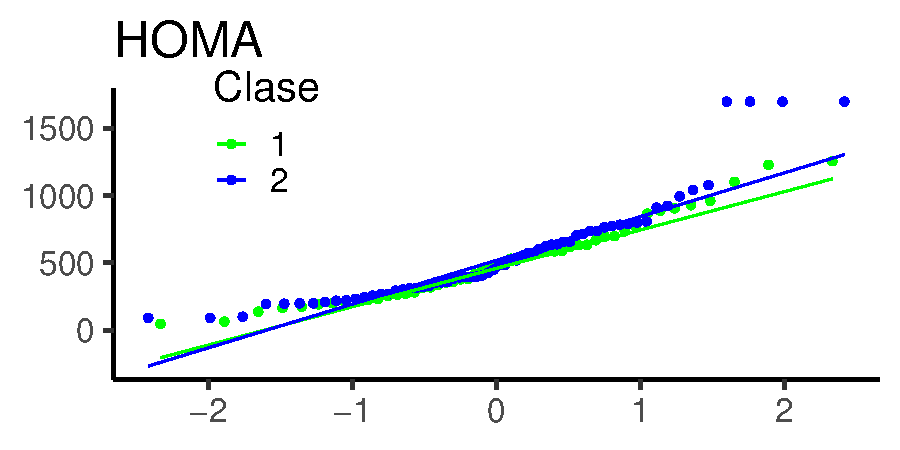
\includegraphics[width = 0.4\linewidth]{../R/images/qq9.pdf}
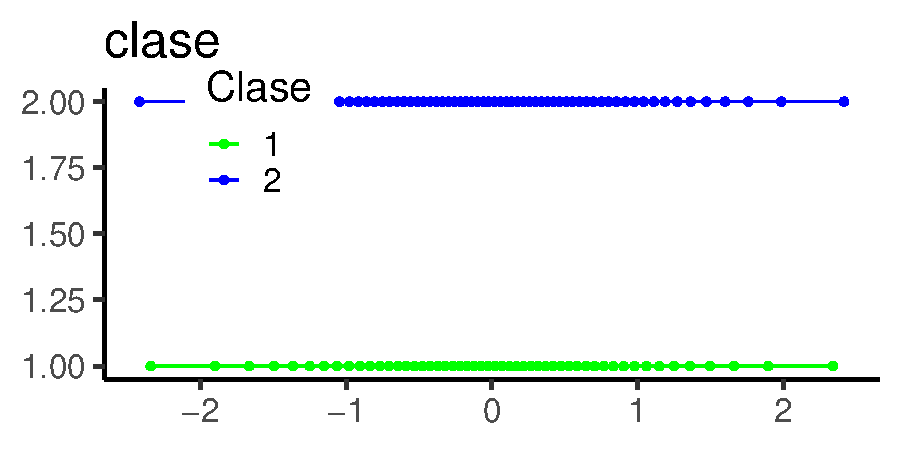
\includegraphics[width = 0.4\linewidth]{../R/images/qq10.pdf}
\figcaption{QQplots R.}
\label{fig:densR}
\end{figure}

\lstinputlisting[
	linerange = {8-18},
	caption = {[C\'odigo R generador de los QQplots.]
	\lstcaption{C\'odigo R generador de los QQplots.}},
	]{../R/src/qqplot.r}
\newpage
\seccion{Corrplot}
\vfill
\begin{figure}[h]
\centering
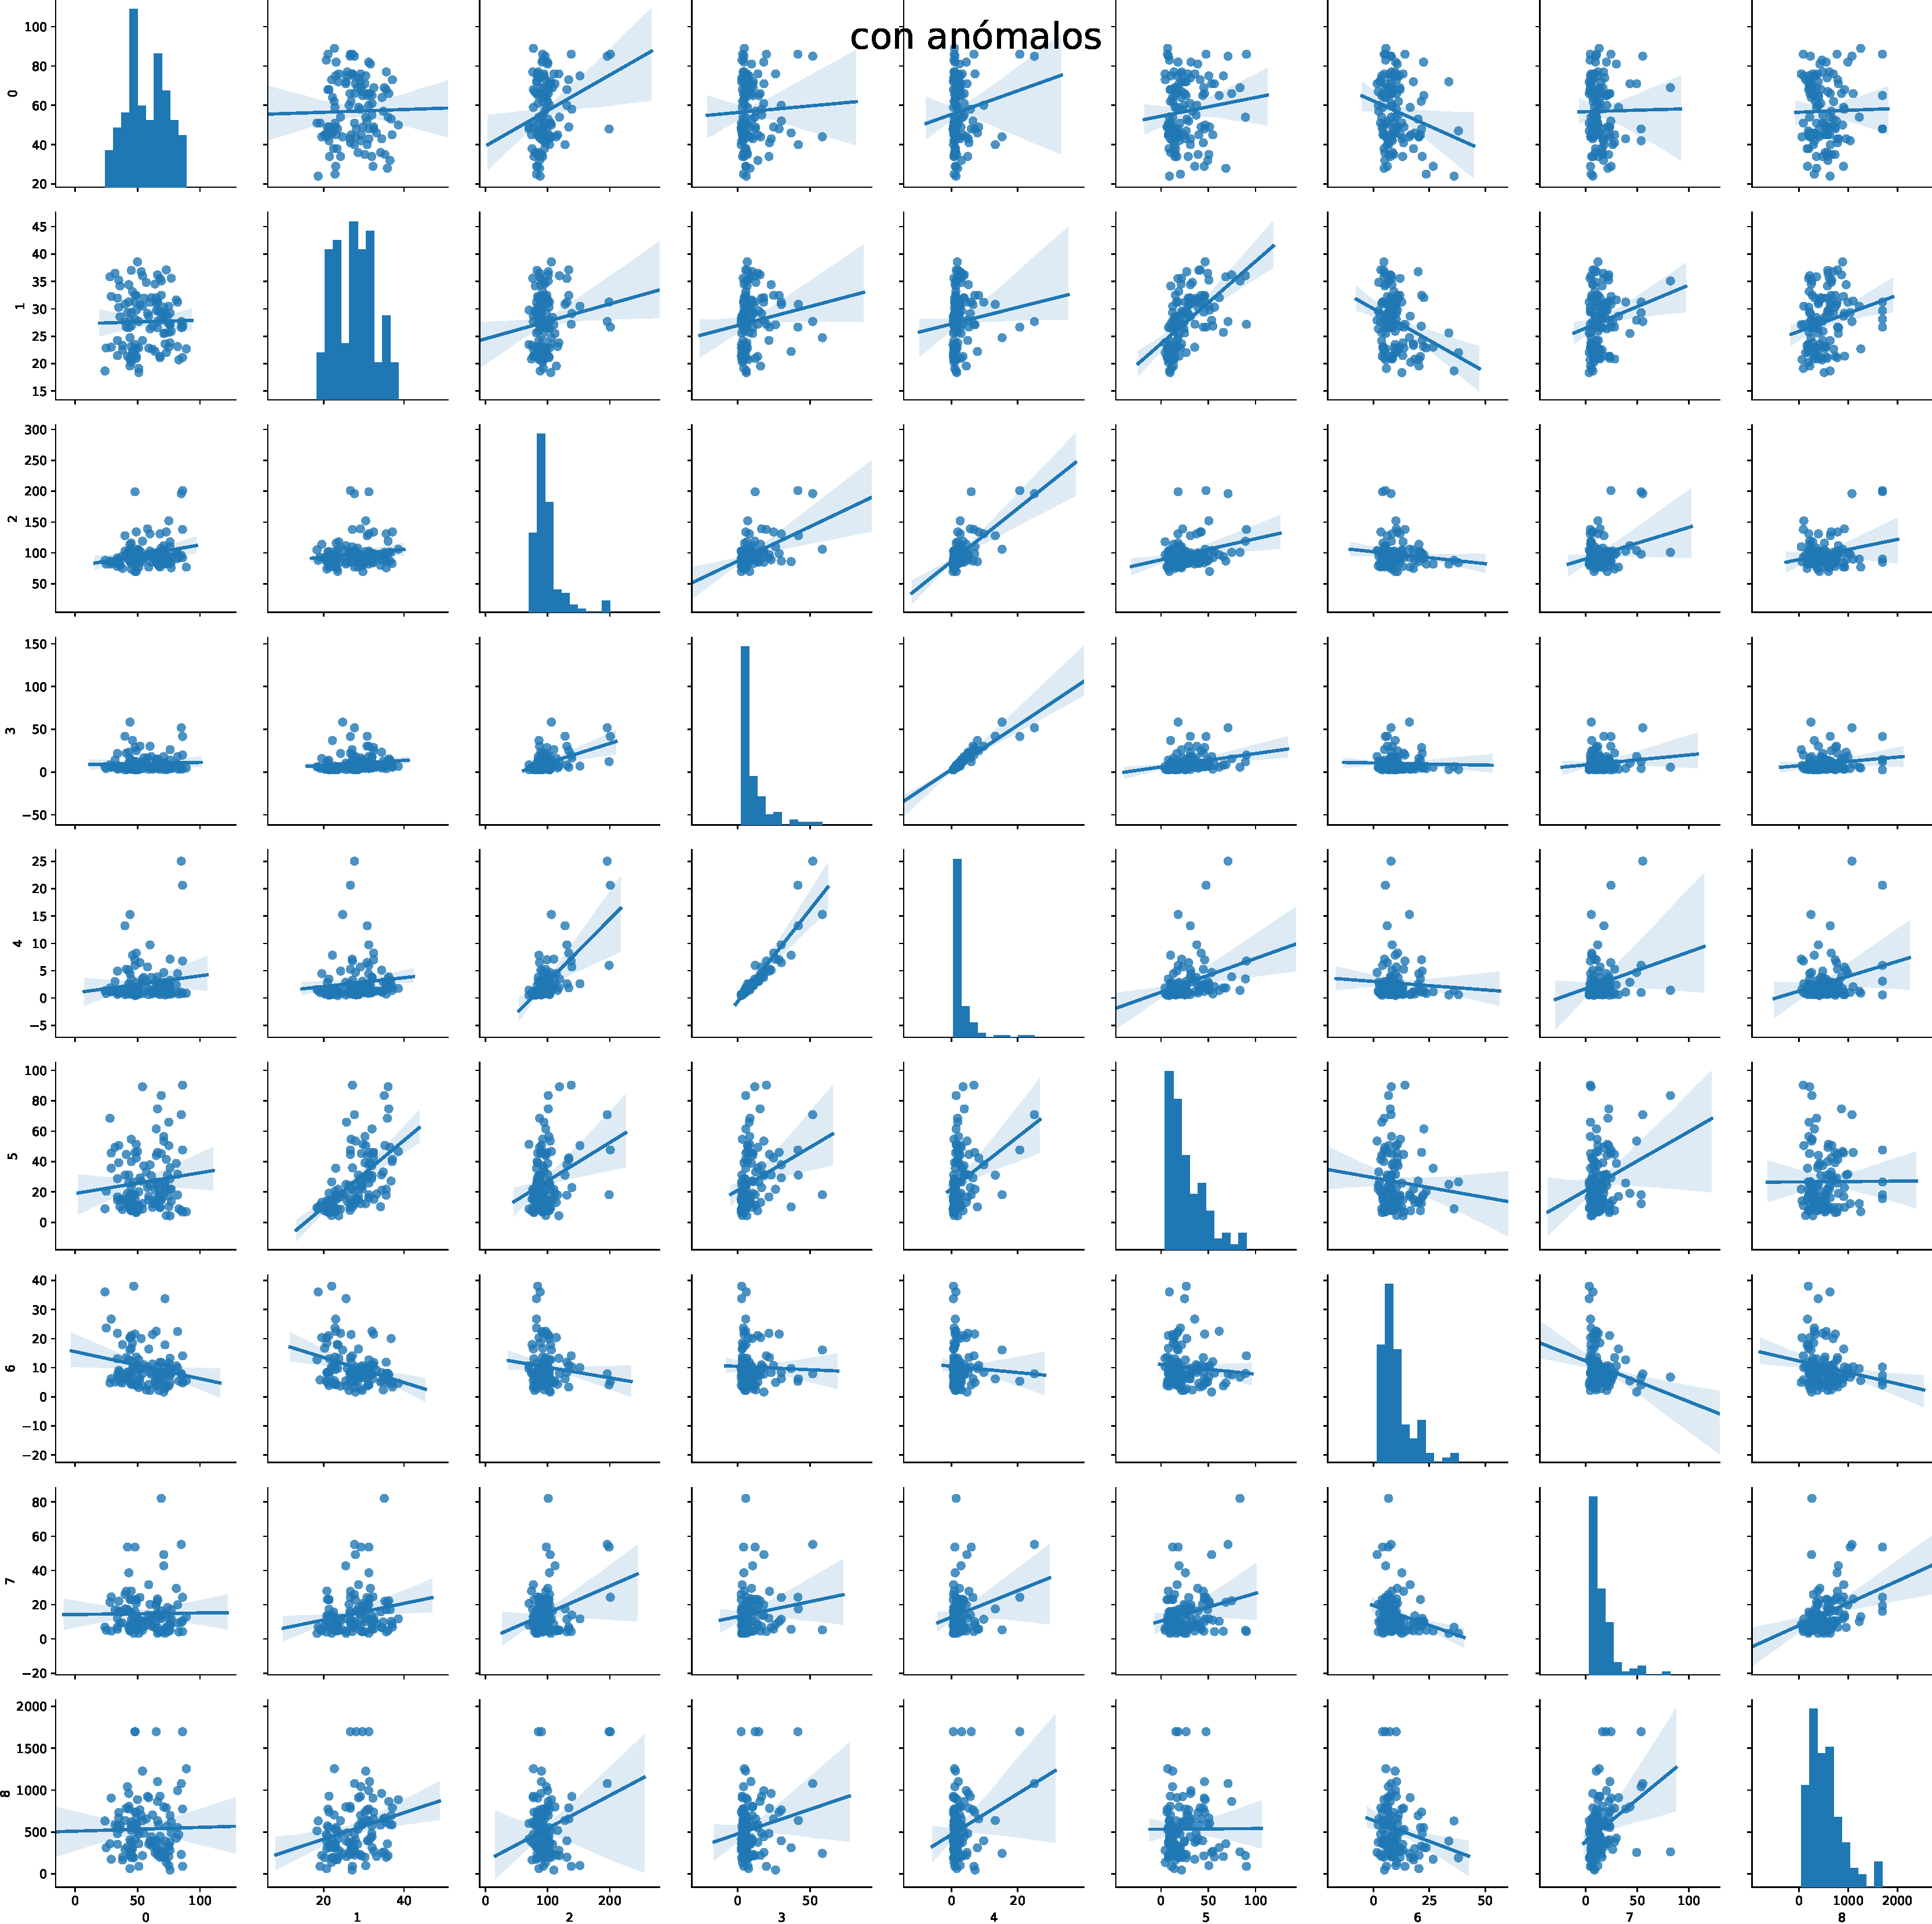
\includegraphics[width = \linewidth]{../python/images/corrp.pdf}
\figcaption{Corrplot Python para datos con anomalias.}
\label{fig:cps}
\end{figure}
\vfill
\lstinputlisting[
	linerange = {13-18},
	caption = {[C\'odigo Python generador de los corrplots con datos an\'omalos.]
	\lstcaption{C\'odigo Python generador de los corrplots con datos an\'omalos.}},
	]{../python/src/corrplot.py}
\vfill

\newpage

\phantom{}
\vfill

\begin{figure}[h!]
\centering
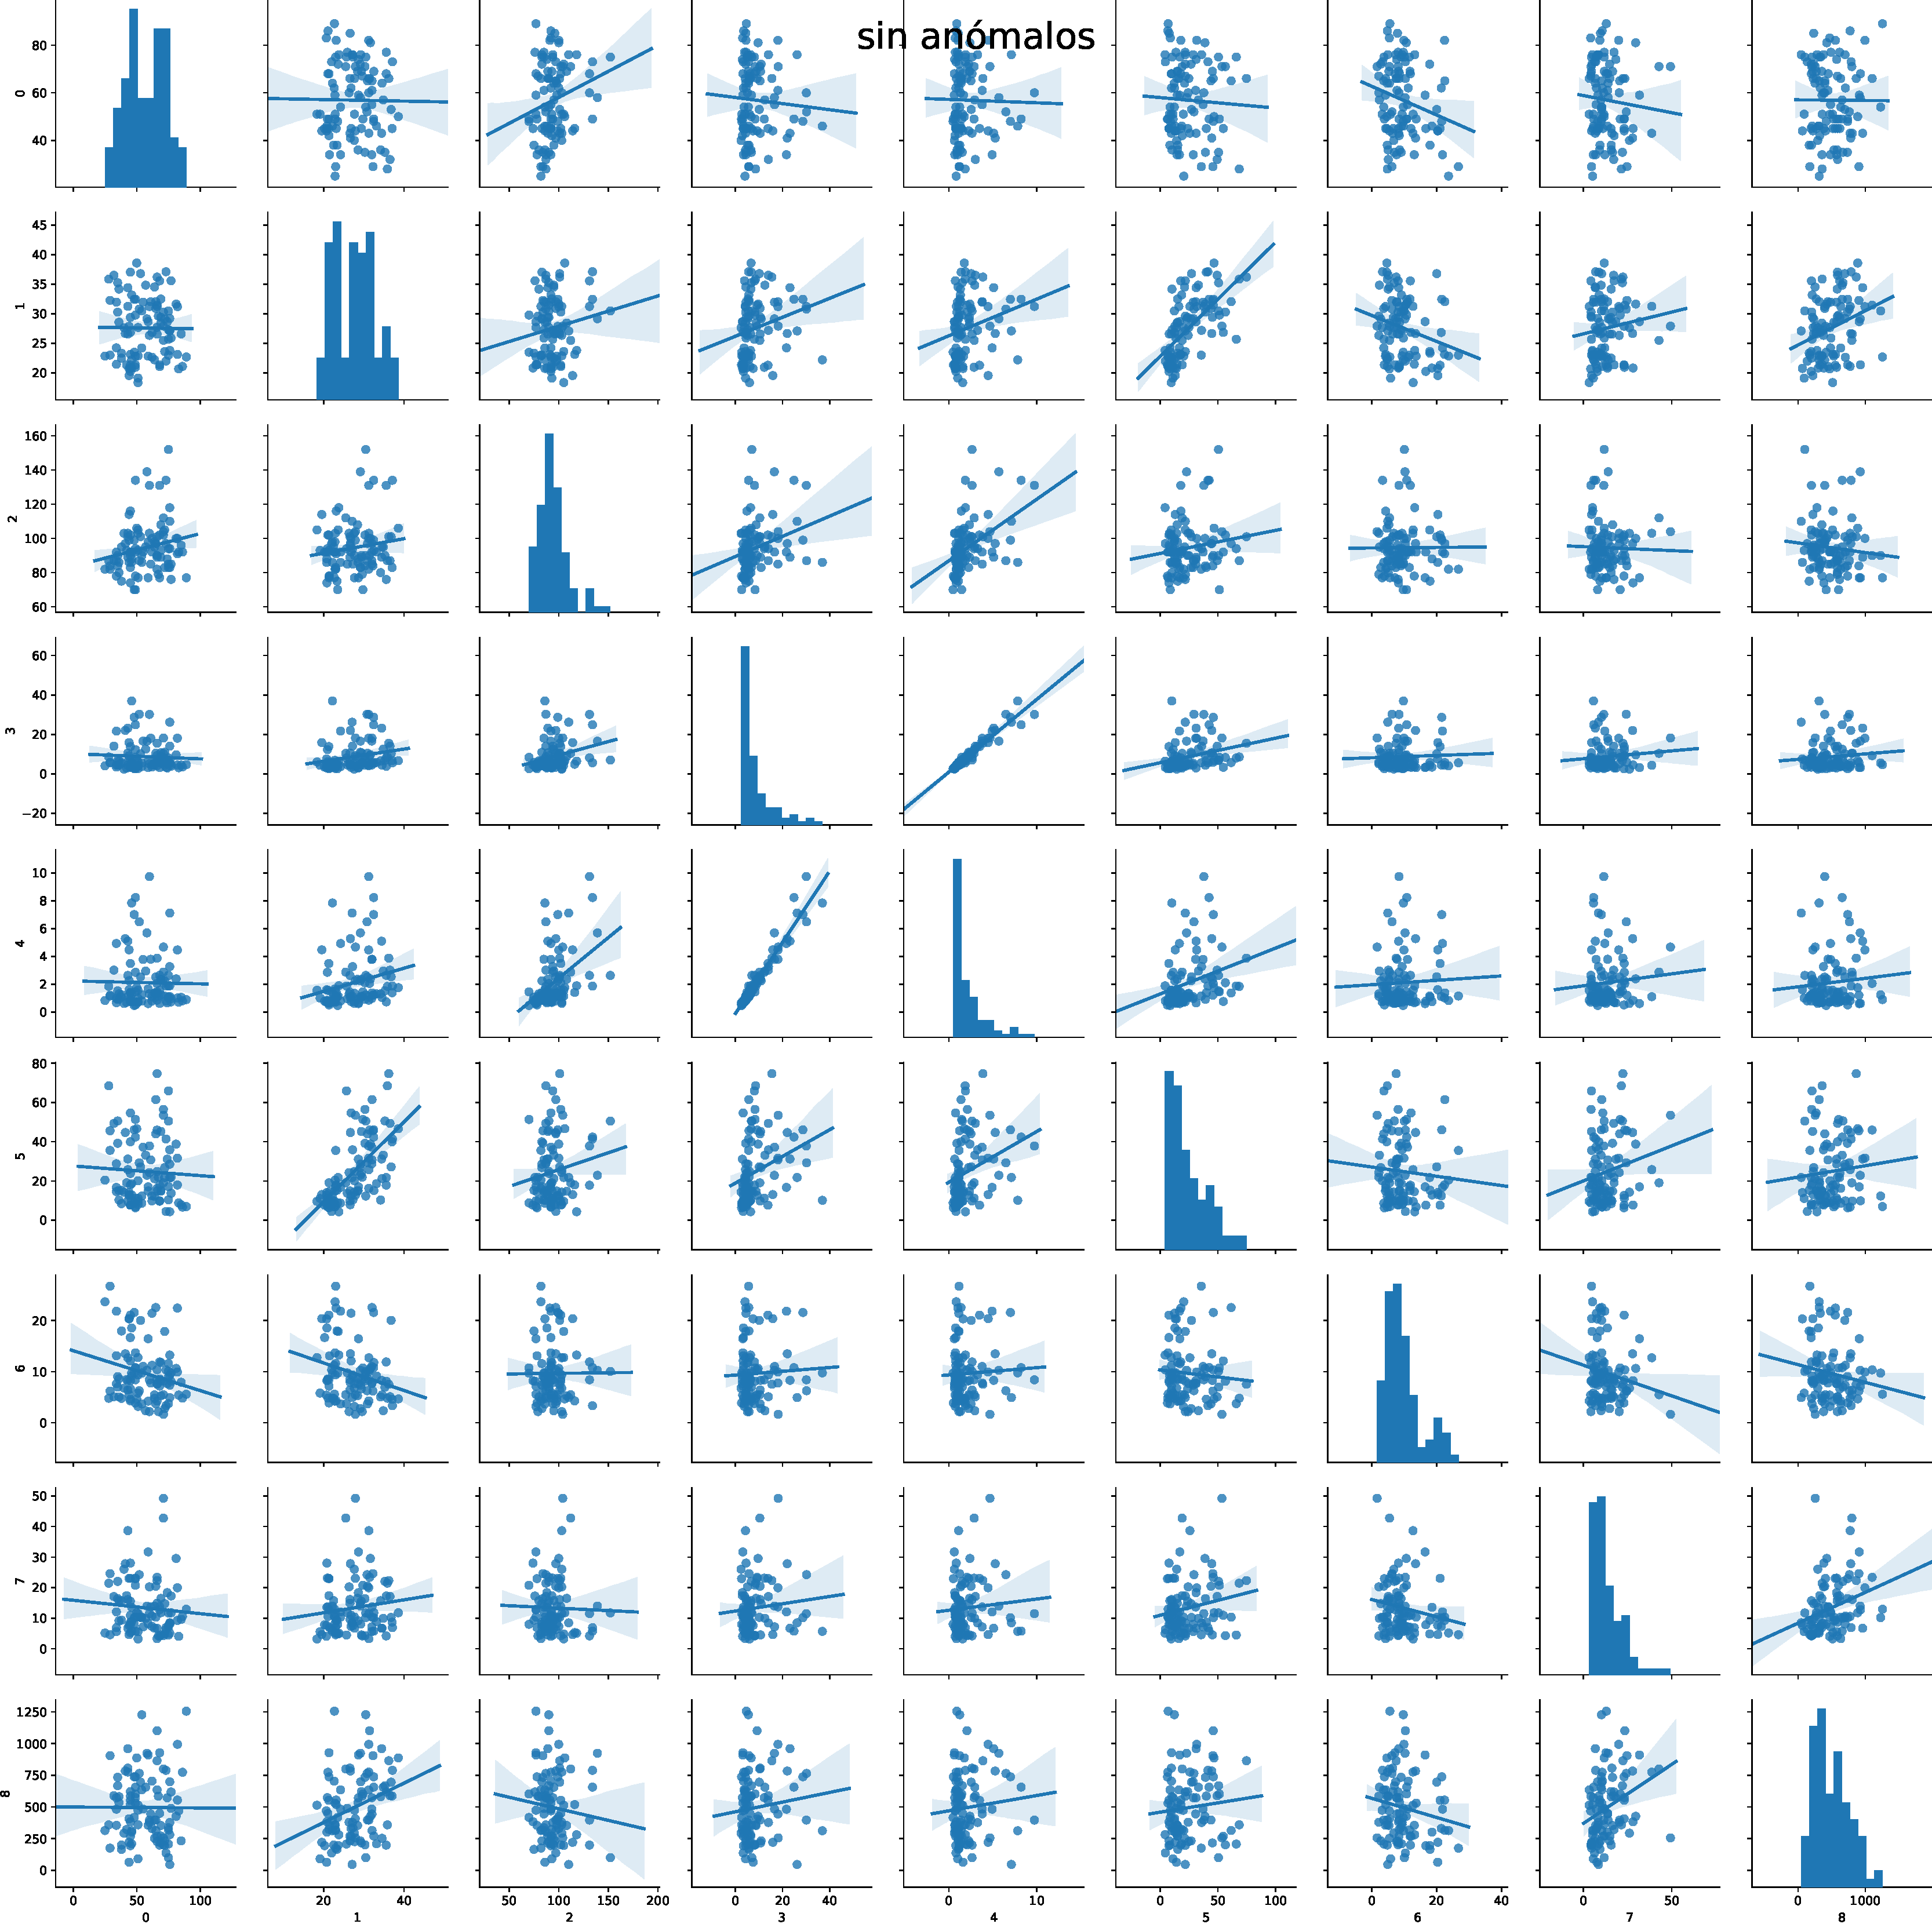
\includegraphics[width = \linewidth]{../python/images/corrp1.pdf}
\figcaption{Corrplot Python para datos sin anomalias.}
\label{fig:cp1s}
\end{figure}

\vfill

\newpage
\begin{figure}[h]
\centering
\includegraphics[width = \linewidth]{../R/images/corrplot.pdf}
\figcaption{Corrplot R para datos con anomalias.}
\label{fig:corrR}
\end{figure}

\lstinputlisting[
	linerange = {9-18},
	caption = {[C\'odigo R generador de los corrplots.]
	\lstcaption{C\'odigo R generador de los corrplots.}},
	]{../R/src/corrplot.r}

\newpage
\begin{figure}[h]
\centering
\includegraphics[width = \linewidth]{../R/images/corrplot1.pdf}
\figcaption{Matriz de correlaciones en R.}
\label{fig:corrR1}
\end{figure}

\newpage

\seccion{Filter Methods}

\lstinputlisting[
	linerange = {16 - 32},
	caption = {[Aplicaci\'on m\'etodos \textit{filter} de selecci\'on caracter\'isticas.]
	\lstcaption{Aplicaci\'on m\'etodos \textit{filter} de selecci\'on caracter\'isticas.}},
	]{../python/src/featureselection.py}

\begin{lstlisting}[
	caption = {[Ranking de variables seg\'un los m\'etodos filter.]
	{\lstcaption{Ranking de variables seg\'un los m\'etodos filter.}}},
	]
[4 5 9 6 7 3 1 8 2] -> fscore
[1 9 8 7 6 5 4 2 3] -> relieff
[3 4 1 1 1 2 3 6 1] -> diferencias
2.4444444444444446  -> media
\end{lstlisting}

\newpage
\begin{lstlisting}[
	caption =  {[Ranking de variables seg\'un distintos m\'etodos en R.]
	{\lstcaption{Ranking de variables seg\'un distintos m\'etodos en R.}}},
	]
# Fscore
library (PredPsych)
rank (fscore (datos, 10, 1:9))
#  age  leptin  bmi adiponectin  glucose  resistin  insulin MCP1  HOMA
#    3       5    9           7        8         2        1    6     4

# Relieff
brary (CORElearn)
rank (attrEval (as.factor (clase)~., datos, 'Relief'))
#  age  leptin  bmi adiponectin  glucose  resistin  insulin  MCP1  HOMA
#    9       7    8           2        4         5        1     6     3

# Algunos de los posibles metodos
for (i in infoCore (what = "attrEval")){
    cat (i, '\r\t\t', unname (rank (attrEval (as.factor (clase)~., datos, i))),'\n')
}
# ReliefFequalK    9 3 8 4 6 5 2 7 1
# ReliefFexpRank   8 5 9 3 6 4 1 7 2
# ReliefFbestK     9 7 8 3 4 5 1 6 2
# Relief           9 7 8 2 4 5 1 6 3
# InfGain          7 4 9 5 8 2 1 6 3
# GainRatio        9 2 8 7 6 4.5 1 3 4.5
# MDL              7 4 9 5 8 3 1 6 2
# Gini             7 4 9 5 8 3 1 6 2
# MyopicReliefF    6 4 9 5 7 3 1 8 2
# Accuracy         6 4 9 5 7 3 1.5 8 1.5
# ReliefFmerit     8 3 9 5 6 4 1 7 2
# ReliefFdistance  8 4 9 5 6 3 1 7 2
# ReliefFsqrDistan 8 4 9 5 6 3 1 7 2
# DKM              7 3 9 6 8 2 1 5 4
# ReliefFexpC      8 5 9 3 6 4 1 7 2
# ReliefFavgC      8 5 9 3 6 4 1 7 2
# ReliefFpe        8 5 9 3 6 4 1 7 2
# ReliefFpa        8 5 9 3 6 4 1 7 2
# ReliefFsmp       8 5 9 3 6 4 1 7 2
# GainRatioCost    9 2 8 7 6 4.5 1 3 4.5
# DKMcost          7 4 9 5 8 3 2 6 1
# 		.  .  .
\end{lstlisting}

\newpage
\seccion{Wrapper Methods}

\lstinputlisting[
	linerange = {38 - 58},
	caption = {[Aplicaci\'on m\'etodos \textit{wrapper} de selecci\'on caracter\'isticas.]
	\lstcaption{Aplicaci\'on m\'etodos \textit{wrapper} de selecci\'on caracter\'isticas.}},
	]{../python/src/featureselection.py}

\begin{lstlisting}[
	caption = { [Resultados Python del filtrado mediante wrappers.]
	{\lstcaption{Resultados Python del filtrado mediante wrappers.}}},
	]
0.7054545454545454
Sequential Forward  Selection ('leptin', 'bmi', 'glucose', 'MCP1')

0.7094949494949495
Sequential Backward Selection ('leptin', 'bmi', 'glucose', 'insulin')
\end{lstlisting}
\newpage

\begin{lstlisting}[
	caption = {[Resultados R del filtrado mediante wrappers.]
	{\lstcaption{Resultados R del filtrado mediante wrappers.}}},
	]
# Sequential Feature Selector
library (mlr)
# Forward
sfs <- selectFeatures (
      learner    = makeLearner      ('classif.knn', k = 9, l = 3),
      task       = makeClassifTask  (data = datos, target = 'clase'),
      resampling = makeResampleDesc ("CV", iter = 50),
      control    = makeFeatSelControlSequential (method = "sfs", maxit = 100L))
# FeatSel result:
# Features (4): age, leptin, bmi, MCP1
# mmce.test.mean=0.1833333

# Backward
sbs <- selectFeatures (
      learner    = makeLearner      ('classif.knn', k = 9, l = 3),
      task       = makeClassifTask  (data = datos, target = 'clase'),
      resampling = makeResampleDesc ("CV", iter = 50),
      control    = makeFeatSelControlSequential (method = "sbs", maxit = 100L))
# FeatSel result:
# Features (4): age, leptin, bmi, MCP1
# mmce.test.mean=0.1800000
\end{lstlisting}

\begin{lstlisting}[
	caption =   {[M\'etodo Boruta \textit{wrapper} de Random Forest R.]
	{\lstcaption{M\'etodo Boruta \textit{wrapper} de Random Forest R.}}},
	]
# esto es extra
library (Boruta)
Boruta (as.factor (clase)~., datos, maxRuns = 101) -> borutaout

# Boruta performed 100 iterations in 4.317041 secs.
#  5 attributes confirmed important: age, bmi, glucose, leptin, MCP1;
#  3 attributes confirmed unimportant: HOMA, insulin, resistin;
#  1 tentative attributes left: adiponectin;

pdf ("../images/boruta.pdf")
plot (borutaout, las = 2, xlab = '', main = 'Boruta Variable Importance')
dev.off ()
\end{lstlisting}

\newpage
\phantom{}
\vfill
\begin{figure}[h]
\centering \includegraphics[width = 0.8\linewidth]{../R/images/boruta.pdf} \figcaption{Representación gráfica de la importancia de las variables
	seleccionadas por Boruta.}
\label{fig:bor}
\end{figure}
\vfill
\phantom{}
\newpage
\seccion{PCA}
\vspace{1cm}
\lstinputlisting[
	linerange = {60-65},
	caption = {[\textit{Principal Component Analysis} Python.]
	\lstcaption{\textit{Principal Component Analysis} Python.}},
	]{../python/src/featureselection.py}
\begin{lstlisting}[
	caption = {[Varianza explicada por componente y suma acumulada Python.]
       {\lstcaption{Varianza explicada por componente y suma acumulada Python.}}},
	]
[0.29146865 0.18490568 0.14125105 0.11727276 0.08486126 0.07999359
 0.06636991 0.03254865 0.00132847]
[0.29146865 0.47637432 0.61762537 0.73489813 0.81975939 0.89975298
0.96612289 0.99867153 1.        ]
\end{lstlisting}

\lstinputlisting[
	linerange = {7-8},
	caption = {[\textit{Principal Component Analysis} R.]
	\lstcaption{\textit{Principal Component Analysis} R.}},
	]{../R/src/pca.r}

\begin{lstlisting}[
	caption = {[Varianza explicada por componente y suma acumulada R.]
       {\lstcaption{Varianza explicada por componente y suma acumulada R.}}},
	]
Importance of components:
                PC1    PC2    PC3   PC4   PC5    PC6    PC7     PC8     PC9
Std deviation   1.7475 1.2393 1.082 1.048 0.8528 0.8144 0.66261 0.53101 0.17555
Propor. of Var. 0.3393 0.1707 0.130 0.122 0.0808 0.0737 0.04878 0.03133 0.00342
Cum. Var.       0.3393 0.5100 0.640 0.762 0.8428 0.9165 0.96525 0.99658 1.00000
\end{lstlisting}

\subseccion{Pareto}
\vspace{0.9cm}
\lstinputlisting[
	linerange = {93-100},
	caption = {[C\'odigo generador del diagrama de Pareto en Python.]
	\lstcaption{C\'odigo generador del diagrama de Pareto en Python.}},
	]{../python/src/featureselection.py}

\lstinputlisting[
	linerange = {12-32},
	caption = {[C\'odigo generador del diagrama de Pareto en R.]
	\lstcaption{C\'odigo generador del diagrama de Pareto en R.}},
	]{../R/src/pca.r}


\begin{figure}[h]
\centering
\includegraphics[width = 0.49\linewidth]{../python/images/pareto.pdf}
\includegraphics[width = 0.49\linewidth]{../R/images/pareto.pdf}
	\figcaption{Diagrama de Pareto en Python y R.}
\label{fig:pareto}
\end{figure}

\newpage
\subseccion{Biplot}

\begin{figure}[h]
\centering
\includegraphics[width = 0.7\linewidth]{../python/images/biplotpca.pdf}
\figcaption{Biplot Python.}
\label{fig:biplotP}
\end{figure}

\lstinputlisting[
	linerange = {71-89},
	caption = {[C\'odigo generador del Biplot en Python.]
	\lstcaption{C\'odigo generador del Biplot en Python.}},
	]{../python/src/featureselection.py}

\newpage
\begin{figure}[h]
\centering
\includegraphics[width = 0.8\linewidth]{../R/images/biplot.pdf}
\figcaption{Biplot R.}
\label{fig:biplotR}
\end{figure}
\lstinputlisting[
	linerange = {34-48},
	caption = {[C\'odigo generador del Biplot en R.]
	\lstcaption{C\'odigo generador del Biplot en R.}},
	]{../R/src/pca.r}
\newpage
\seccion{Modelos de Clasificación}

\subseccion{Clasificación Lineal}
\vfill
\lstinputlisting[
	linerange = {19-36},
	caption = {[Python validaci\'on del modelo lineal.]
	\lstcaption{Python validaci\'on del modelo lineal.}},
	]{../python/src/clasificadorlineal1.py}
\vfill
\begin{lstlisting}[
	caption = {[Python validaci\'on seg\'un distintos m\'etodos de partici\'on.]
       {\lstcaption{Python validaci\'on seg\'un distintos m\'etodos de partici\'on.}}},
	]
Linear puntuacion CV media: 0.75 std: 0.13
Linear puntuacion KF media: 0.75 std: 0.10
Linear puntuacion SS media: 0.71 std: 0.14
Linear puntuacion LO media: 0.76 std: 0.43
\end{lstlisting}
\vfill

\newpage

\phantom{}
\vfill
\lstinputlisting[
	linerange = {14-37},
	mathescape=false,
	caption = {[R an\'alisis lineal discriminante.]
	\lstcaption{R an\'alisis lineal discriminante.}},
	]{../R/src/clasificacion.r}
\vfill
\begin{lstlisting}[
	caption = {[R puntuaci\'on de mil evaluaciones.]
       {\lstcaption{R puntuaci\'on de mil evaluaciones.}}},
	]
	  vars   n  mean   sd median trimmed  mad  min  max range  skew
ldascores    1 1000 0.72 0.08   0.73    0.72 0.10 0.47 0.97  0.50 -0.09
\end{lstlisting}
\vfill

\newpage
\subseccion{Clasificación Cuadrática}
\vfill
\lstinputlisting[
	linerange = {40-58},
	caption = {[Python validaci\'on del modelo cuadr\'atico.]
	\lstcaption{Python validaci\'on del modelo cuadr\'atico.}},
	]{../python/src/clasificadorlineal1.py}
\vfill
\begin{lstlisting}[
	caption = {[Python validaci\'on seg\'un distintos m\'etodos de partici\'on.]
       {\lstcaption{Python validaci\'on seg\'un distintos m\'etodos de partici\'on.}}},
	]
Quadratic puntuacion CV media: 0.66 std: 0.19
Quadratic puntuacion KF media: 0.76 std: 0.09
Quadratic puntuacion SS media: 0.76 std: 0.14
Quadratic puntuacion LO media: 0.73 std: 0.44
\end{lstlisting}
\vfill
\newpage
\phantom{}
\vfill
\lstinputlisting[
	linerange = {42-63},
	mathescape=false,
	caption = {[R an\'alisis cuadr\'atico discriminante.]
	\lstcaption{R an\'alisis cuadr\'atico discriminante.}},
	]{../R/src/clasificacion.r}
\vfill
\begin{lstlisting}[
	caption = {[R puntuaci\'on de mil evaluaciones.]
       {\lstcaption{R puntuaci\'on de mil evaluaciones.}}},
	]
     vars        n mean   sd median trimmed  mad  min  max range  skew
qdascores    2 1000 0.69 0.07   0.70    0.69 0.10 0.43 0.87  0.43 -0.17
\end{lstlisting}
\vfill

\newpage
\subseccion{Clasificación KNN}
\vfill

\lstinputlisting[
	linerange = {15-33},
	caption = {[Python validaci\'on del modelo KNN.]
	\lstcaption{Python validaci\'on del modelo KNN.}},
	]{../python/src/clasificadorknn.py}

\vfill
\begin{lstlisting}[
	caption = {[Python validaci\'on seg\'un distintos m\'etodos de partici\'on.]
       {\lstcaption{Python validaci\'on seg\'un distintos m\'etodos de partici\'on.}}},
	]
KNN puntuacion CV media: 0.47 std: 0.12
KNN puntuacion KF media: 0.47 std: 0.15
KNN puntuacion SS media: 0.47 std: 0.13
KNN puntuacion LO media: 0.43 std: 0.50
\end{lstlisting}
\vfill

\newpage
\phantom{}
\vfill
\lstinputlisting[
	linerange = {66-89},
	mathescape=false,
	caption = {[R \textit{K nearest neighbours}.]
	\lstcaption{R \textit{K nearest neighbours}.}},
	]{../R/src/clasificacion.r}
\vfill
\begin{lstlisting}[
	caption = {[R puntuaci\'on de mil evaluaciones.]
       {\lstcaption{R puntuaci\'on de mil evaluaciones.}}},
	]
     vars        n mean   sd median trimmed  mad  min  max range  skew
knnscores    3 1000 0.66 0.07   0.67    0.66 0.05 0.43 0.90  0.47 -0.07
\end{lstlisting}
\vfill
\newpage

\seccion{Postámbulo}

\begin{figure}[h]
\centering
\includegraphics[width = 0.7\linewidth]{../python/images/knn.pdf}
\figcaption{Rendimineto decreciente según aumenta el número de vecinos.}
\label{fig:knn}
\end{figure}

\begin{figure}[h]
\centering
\includegraphics[width = 0.9\linewidth]{../R/images/scores.pdf}
\figcaption{Comparación de mil evaluaciones de cada uno de los métodos de clasificación en R.}
\end{figure}

\lstinputlisting[
	linerange = {37-55},
	caption = {[Evoluci\'on de puntuaci\'on seg\'un n\'umero de vecinos.]
	\lstcaption{Evoluci\'on de puntuaci\'on seg\'un n\'umero de vecinos.}},
	]{../python/src/clasificadorknn.py}



\end{document}
